%\documentclass{book}\usepackage{sjtfonts}\usepackage{includegraphics}\usepackage{alltt}\usepackage{latexsym}
%\usepackage{array}
%\begin{document}\input{defs0}%		miradefs.tex 		    June 1994

% opening and closing a quoted Miranda section

\newcommand{\mira}{\noindent\hrulefill\nopagebreak\so}
\newcommand{\arim}{\nopagebreak\st\hrulefill\\}

% backslash in the Miranda environment
% Only feasible approach is to use \verb+\+
% in line!

%\newcommand{\bs}{$\mi\backslash\!\!$}
%\newcommand{\lbs}{\mbox{\verb+\+}}

% ignoring part of the input

\newcommand{\ignore}[1]{}

% a blank line in a Miranda section

\newcommand{\bl}{\mbox{\ }}

% Signalling a diffculty.

\definecolor{light-gray}{gray}{0.95}

\newcommand{\beware}[2]
 {\medskip\noindent\colorbox{light-gray}{\parbox{\textwidth}
 {\mbox{\large\textbf{#1}} \medskip\noindent\\ #2}\medskip\noindent}}

% Subscripting in Miranda text
\newcommand{\subscr}[2]{\mbox{${\mbox{\texttt{#1}}}_{\mbox{\texttt{#2}}}$}}

%\newcommand{\subscr}[2]{\mbox{${\mbox{\mi #1}}_{\mbox{\smtt #2}}$}}
\newcommand{\aone}{\subscr{a}{1}}
\newcommand{\atwo}{\subscr{a}{2}}
\newcommand{\ak}{\subscr{a}{k}}

\newcommand{\aoneone}{\subscr{a}{1,1}}

\newcommand{\eone}{\subscr{e}{1}}
\newcommand{\etwo}{\subscr{e}{2}}
\newcommand{\ei}{\subscr{e}{i}}
\newcommand{\er}{\subscr{e}{r}}

\newcommand{\fone}{\subscr{f}{1}}
\newcommand{\fl}{\subscr{f}{l}}

\newcommand{\gone}{\subscr{g}{1}}
\newcommand{\gtwo}{\subscr{g}{2}}
\newcommand{\gi}{\subscr{g}{i}}
\newcommand{\gr}{\subscr{g}{r}}

\newcommand{\hone}{\subscr{h}{1}}
\newcommand{\hl}{\subscr{h}{l}}

\newcommand{\pone}{\subscr{p}{1}}
\newcommand{\ptwo}{\subscr{p}{2}}
\newcommand{\pk}{\subscr{p}{k}}

\newcommand{\qone}{\subscr{q}{1}}
\newcommand{\qtwo}{\subscr{q}{2}}
\newcommand{\qk}{\subscr{q}{k}}

\newcommand{\rone}{\subscr{r}{1}}
\newcommand{\rtwo}{\subscr{r}{2}}

\newcommand{\tone}{\subscr{t}{1}}
\newcommand{\ttwo}{\subscr{t}{2}}
\newcommand{\tn}{\subscr{t}{n}}

\newcommand{\vone}{\subscr{v}{1}}
\newcommand{\vtwo}{\subscr{v}{2}}
\newcommand{\vn}{\subscr{v}{n}}

% for regular expressions

\newcommand{\stone}{\subscr{st}{1}}
\newcommand{\sttwo}{\subscr{st}{2}}
\newcommand{\stn}{\subscr{st}{n}}
\newcommand{\rthree}{\subscr{r}{3}}

\newcommand{\eps}{$\varepsilon$}
\newcommand{\trans}[1]{\stackrel{\mbox{\tt #1}}{\longrightarrow}}



% superscript in Miranda text

\newcommand{\superscr}[2]{\mbox{${\mbox{\mi #1}}^{\mbox{\smtt #2}}$}}

% Not equals in Miranda text

\newcommand{\noteq}{\makebox[0pt][l]{=}/}
\newcommand{\overslash}{\makebox[0pt][l]{/}}

% Definitions in complexity chapter

\newfont{\oldSym}{cmsy10}
\newcommand{\Th}{\boldmath$\oldSym\Theta$}
\newcommand{\pow}[1]{\^{}#1}
\newcommand{\leqq}{$\leq$}
\newcommand{\geqq}{$\geq$}
\newcommand{\lll}{$\ll$}
\newcommand{\eqq}{$\equiv$}
\newcommand{\ltwo}{\subscr{log}{2}}

% Indexing

\newcommand{\minx}[1]{\index{#1@{\ttfamily{}#1}}}


\chapter{Programming with lists}
\chapstart
\label{progLists}


The aim of this chapter is to introduce the operations on lists contained in the prelude and the libraries that come with Haskell 2010. In order to understand the types of these library functions we 
have to examine how generic or \textbf{polymorphic} functions.
Polymorphism is the mechanism by which a Haskell
function can act over more than one type: the \texttt{length} function
on lists can be used over any list type, for instance. 

After doing this we're in a position to review the functions in the prelude, in the Haskell 2010 libraries, and those others which appear on Hackage. All these are reviewed, and in particular we look at how we can discover functions with the type or behaviour that we're looking for.

To make use of these library functions, we then introduce a series of extended exercises to stretch the reader
rather more than the small exercises we have given thus far. These include extensions of the \texttt{Picture} functions and a billing program for a supermarket checkout, which has to produce
a formatted bill from the list of bar codes scanned in at a checkout. Finally we include the example of card games, which shows the importance of \emph{type design} in writing non-trivial programs.


\section{Generic functions: polymorphism}
\label{poly}
\index{polymorphism|(}
\index{genericity}
 
Before looking in detail at the functions on lists provided in the
Haskell prelude and libraries
we need to look at the idea of
\textbf{polymorphism}, which literally means `has many shapes'. A
function is polymorphic if it `has many types', and this is the case
for many list-manipulating functions. An example is the
\texttt{length}\minx{length}
function, which returns the length of a list, an \texttt{Int}. This function
can be applied to any
type of list, so that we can say
\begin{alltt}
length :: [Bool] -> Int
length :: [[Char]] -> Int
\end{alltt}
and so forth.
How do we write down a type for \texttt{length} which encapsulates this?
We say
\begin{alltt}
length :: [a] -> Int
\end{alltt}
where \texttt{a} is a \textbf{type variable}\index{type
variable}\index{variable!type}. Any identifier beginning with a small letter
can be used as a type variable;  conventionally, letters from the beginning of the
alphabet, \texttt{a}, \texttt{b}, \texttt{c}, \ldots\ are
used.\index{conventions!type variable names}
Just as in the definition
\begin{alltt}
square x = x*x
\end{alltt}
the variable \texttt{x} stands for an arbitrary value, 
so a type variable stands for an {\em
arbitrary type}, and so we can see all the types like 
\begin{alltt}
[Bool] -> Int          [[Char]] -> Int
\end{alltt}
as coming about by replacing the variable \texttt{a} by particular
types: here \texttt{Bool} and \texttt{[Char]}. 

Types like \texttt{[Bool] -> Int}
are called \textbf{instances}\index{instance}\index{type!instance} of the type
\texttt{[a] -> Int}, and because every type for \texttt{length} is an instance of
\texttt{[a] -> Int} we call this type the \textbf{most general type}
\index{type!most general} for \texttt{length}.
The type of the function to join together two lists, \texttt{++}, is 
\begin{alltt}\minx{++}
[a] -> [a] -> [a]
\end{alltt} 
The variable \texttt{a} stands for `an arbitrary type', but we should be
clear that all the \texttt{a}'s stand for the same type, just as in 
\begin{alltt}
square x = x*x
\end{alltt}
the \texttt{x}'s all stand for the same (arbitrary) value. Instances of
\texttt{[a]->[a]->[a]} will include 
\begin{alltt}
[Integer]->[Integer]->[Integer]
\end{alltt}
but {\em not\/} the type
\begin{alltt}
[Integer]->[Bool]->[Char]
\end{alltt}
This makes sense: we cannot expect to join a list of numbers and a list
of Booleans to give a string!

On the other hand, the functions \texttt{zip} and \texttt{unzip} convert
between pairs of lists and lists of pairs, and their types involve two
type variables:\minx{zip}\minx{unzip}
\begin{alltt}
zip   :: [a] -> [b] -> [(a,b)]
unzip :: [(a,b)] -> ([a],[b])
\end{alltt}
because the types of the lists being (un)zipped are not related.
Now, instances of the type of \texttt{zip} include
\begin{alltt}
[Integer]->[Bool]->[(Integer,Bool)]
\end{alltt}
where \texttt{a} and \texttt{b} are replaced by different types 
(\texttt{Integer} and \texttt{Bool}, here). It is, of course, possible to
replace both variables by the same type, giving 
\begin{alltt}
[Integer]->[Integer]->[(Integer,Integer)]
\end{alltt}
and the general type \texttt{[a] -> [a] -> [(a,a)]}.



\subsection*{Types and definitions}

How is a polymorphic function defined?\index{function!definition of
polymorphic}\index{polymorphism!function definition}
Consider the definition of the identity function,
\begin{alltt}\minx{id}
id x = x
\end{alltt}
which returns its argument unchanged. In the definition there is nothing
to \textbf{constrain}\index{constraint}\index{type!constraint} 
the type of \texttt{x} -- all we know about \texttt{x} is that it
is returned directly from the function. We know, therefore, that the
output type is the same as the input, and so the most general type will
be
\begin{alltt}
id :: a -> a
\end{alltt}
At work here is the principle that a function's type is as general as possible, 
consistent with the constraints put upon the types by its
definition. In the case of the \texttt{id} function, the only
constraint is that the input and output types are the same.

In a similar way, in defining
\begin{alltt}\minx{fst}
fst (x,y) = x
\end{alltt}
neither \texttt{x} nor \texttt{y} is constrained at all, and so they can
come from different types \texttt{a} and \texttt{b}, giving the type
\begin{alltt}
fst :: (a,b) -> a
\end{alltt}
A final example is given by 
\begin{alltt}
mystery (x,y) = if x then 'c' else 'd'
\end{alltt}
Here we see that \texttt{x} is used as a \texttt{Bool} in the 
\texttt{if x then ...}, whereas
\texttt{y} is not used at all, and so is not constrained in the definition,
giving \texttt{mystery} the type
\begin{alltt}
(Bool,a) -> Char
\end{alltt}
We shall examine the definitions of many of the \texttt{Prelude} and library functions in 
Chapter \ref{defFunLists}, and see there that, as outlined above, a function or other object
will have as general as possible a type, consistent with the constraints put upon the types by its
definition. We look in more depth at the mechanics of type checking in
Chapter \ref{types}.

GHCi can be used to give the most general type of a function definition,
using the \texttt{:type}\index{type@\texttt{:type}} command. If you have
given a type declaration for the function, this can be commented out
before asking for the type.

\subsection*{Polymorphism and overloading}
\index{polymorphism!and overloading}
\index{overloading!and polymorphism}

Polymorphism and overloading are both mechanisms by which the same
function name can be used at different types, but they have an
important difference.

A polymorphic function like \texttt{fst} has the same definition, namely
\begin{alltt}
fst (x,y) = x
\end{alltt}
at all types, so that it is the \textbf{same} function at all its
instances.

On the other hand, an overloaded name like \texttt{==} has different
definitions over different types, so that the same name is being used to 
mean \textbf{different} but similar functions at different types. For
example, \texttt{==} over \texttt{Integer} is built in, whereas over pairs
it will be defined by
\begin{alltt}
(n,m) == (p,q)
  = (n==p) \&\& (m==q)
\end{alltt}
More details about overloading can be found in Chapter \ref{typeClasses}.

\begin{exercises}

\item
Give the most general types for the functions \texttt{snd} and
\texttt{sing} defined by
\begin{alltt}
snd (x,y) = y
sing x = [x]
\end{alltt}

\item
Explain why 
\begin{alltt}
[[a]] -> [[a]]
\end{alltt}
is a type for \texttt{id} but why it is not the most general type
for this function.

\item
Earlier in the chapter we saw the example of 
\begin{alltt}
shift :: ((Integer,Integer),Integer) -> (Integer,(Integer,Integer))
shift ((x,y),z) = (x,(y,z))
\end{alltt}
What is the most general type for \texttt{shift}, if the type
declaration is omitted?
\index{polymorphism|)}

\end{exercises}




\section{Haskell list functions in the \texttt{Prelude}} 
\markright{Haskell list functions in the \texttt{\runinghead Prelude}}
\index{lists!prelude functions|(}

\begin{figure}
\minx{:}\minx{++}\minx{"!"!}\minx{concat}\minx{length}\minx{head}\minx{last}\minx{tail}
\minx{init}\minx{replicate}\minx{take}\minx{drop}\minx{splitAt}\minx{reverse}\minx{zip}\minx{unzip}
\centering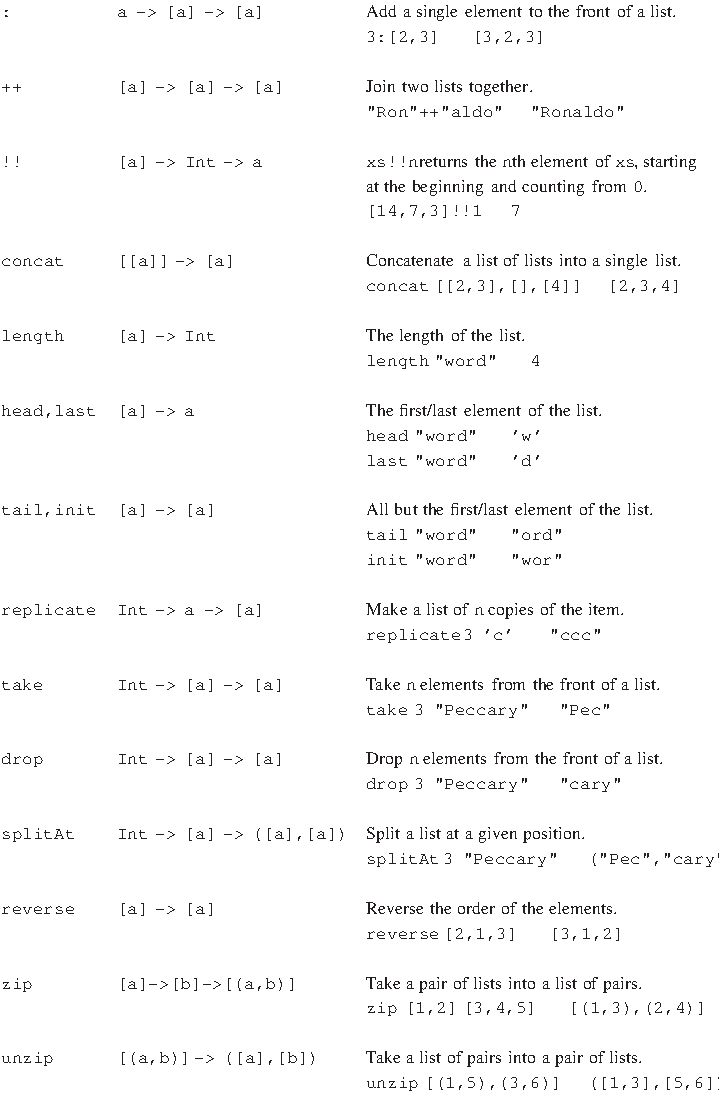
\includegraphics{Pictures/fig5-1.pdf}
\caption{Some polymorphic list operations from \texttt{Prelude.hs}.}
\label{polyListOps}\index{Peccary, Greggery}\index{Greggery Peccary|see{Peccary, Greggery}}
\end{figure}

Armed with the insight provided by the
previous section we can look at the descriptions of the polymorphic list
operations from \texttt{Prelude} given in Figure \ref{polyListOps}. 
In this table we give the name of the
function or operator, its type, a brief description of its effect and an
example, as in the description of \texttt{length}\minx{length}
\begin{center}
\begin{tabular}{>{\ttfamily}p{0.7in}>{\ttfamily}p{1.5in}>{\setlength{\rightskip}{0pt plus 1fil}}p{2.5in}}
length & [a] -> Int & The length of the list.\\
&& \texttt{length "word" \step 4}
\end{tabular}
\end{center}

As well as the polymorphic functions in Figure \ref{polyListOps}, the
standard prelude provides various operations over specific types; some
of these can be seen in Figure \ref{monoListOps}. The types of the
functions
\texttt{sum} and \texttt{product}, which are overloaded, 
will be discussed further in Chapter \ref{typeClasses}.

\begin{figure}
\begin{center}\minx{sum}\minx{product}\minx{and}\minx{or}
\begin{tabular}{>{\ttfamily}p{0.7in}>{\ttfamily}p{1.3in}>{\setlength{\rightskip}{0pt plus
1fil}}p{2.5in}} and & [Bool] -> Bool & The conjunction of a list of Booleans.\\
&& \texttt{and [True,False] \step False}\\ \\
or & [Bool] -> Bool & The disjunction of a list of
Booleans.\\
&& \texttt{or [True,False] \step True}\\ \\
sum & [Integer] -> Integer & The sum of a numeric list.\\
 & [Float] -> Float & \texttt{sum [2,3,4] \step 9}\\ \\
product & [Integer] -> Integer & The product of a numeric list.\\
 & [Float] -> Float & \texttt{product [0.1,0.4 ..\ 1] \step 0.028}
\end{tabular}
\end{center}
\vspace{-10pt}
\caption{Some monomorphic list operations from the \texttt{Prelude}.}
\label{monoListOps}
\vspace{-6pt}
\end{figure}



\subsection*{The importance of types}
\index{type!importance of types}

The single most useful piece of information about a function is its
\textbf{type}, and this is particularly true when we look at the polymorphic types
of functions in a library like Figure \ref{polyListOps}. Suppose we are
looking for a function to make a list from a number of copies of a single element.
It must take the item and a count and give a list, so its type will be 
one of 
\begin{alltt}
Integer -> a -> [a]             a -> Integer -> [a]
\end{alltt}
Looking at Figure \ref{polyListOps} we can quickly locate 
one function, \texttt{replicate}, which does have one of
these types and is indeed the function which we seek. If we want a
function to reverse a list it will have type \mbox{\texttt{[a] -> [a]}} and
although there is more than one function with this type, the search is
very much narrowed by looking at types. We'll see a little later on (page \pageref{hoogle}) that there's a web service called \emph{{hoogle}} to look up functions by type.

This insight is not confined to functional languages, but is of
particular use when a language supports polymorphic or \textbf{generic}
functions and operators as we have seen here.

\subsection*{Further functions}

We have not described all the functions in the prelude for two different
reasons. First, some of the general functions are \textbf{higher-order}
and we postpone discussion of these until Chapter \ref{patternsGen}; secondly,
some of the functions, such as \texttt{zip3}, are obvious variants of
things we have discussed here. Similarly, we have not chosen to
enumerate the functions in the library \texttt{Data.List}; \minx{Data.List}readers should
consult the library file itself, which contains type information and comments
about the effects of the functions, as well as the Haddock documentation for the library: we talk in detail about documentation in the next section.

\begin{figure}[t]
\begin{center}
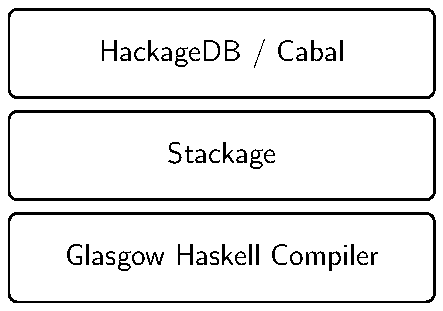
\includegraphics[width=3in]{Pictures/Infrastructure.pdf}
\end{center}
\caption{The Haskell infrastructure}
\label{HaskellInfrastr}
\end{figure}

\index{lists!prelude functions|)}


\section{Finding your way around the Haskell libraries}
\label{HaskellLibs}\index{libraries, finding your way around|(}

\begin{figure}[t]
\beware{A note on \texttt{module} names and exports}{\label{note-names}\index{modules!hierarchical names}\index{pitfalls!module names}
Module names in Haskell 2010 are ``hierarchical'' in style, and consist of a sequence of identifiers beginning with capital letters, separated with dots. Examples in the standard libraries include \texttt{Foreign.Marshal.Alloc}, \texttt{Data.Bool} and \texttt{Foreign}.
To quote from the report 
\begin{quote}
Module names can be thought of as being arranged in a hierarchy in which appending a new component creates a child of the original module name. For example, the module \texttt{Control.Monad.ST} is a child of the \texttt{Control.Monad} sub-hierarchy. This is purely a convention, however, and not part of the language definition.
\end{quote}
However, that's not quite the end of the story, because some modules are defined in such a way as to (re-)export all their ``children'': an example of this is the module \texttt{Foreign.C} (quoting again from the report)
\begin{quote}
The module \texttt{Foreign.C} combines the interfaces of all modules providing C-specific marshalling support, namely
\begin{alltt}
module Foreign.C.Types 

module Foreign.C.String 

module Foreign.C.Error
\end{alltt}
\end{quote}
while other modules export a subset of that functionality:
\begin{quote}
The module \texttt{Foreign} combines the interfaces of all modules providing language-independent marshalling support, namely
\begin{alltt}
module Data.Bits 

module Foreign.Ptr 

 ...
\end{alltt}
\end{quote}
}
\end{figure}

\begin{figure}[t]
\beware{Packages and Hackage}{\label{package-hackage}\index{HackageDB}\index{package}
\textbf{Hackage} is the standard online repository for Haskell code, bundled up as \textbf{packages}. The simplest package is a collection of Haskell modules, but more complex packages can contain C code, documentation, test cases and so on. Hackage keeps track of dependencies between packages, including which versions of each dependency a package is compatible with.

Combined with Cabal\index{Cabal}, this gives a straightforward way to download and maintain sets of Haskell libraries. Cabal has facilities for package developers and maintainers too, but we confine ourselves to user-facing features here.

\medskip
\textbf{Packages} have a globally unique \textbf{package name} and a \textbf{version number}, such as \texttt{mypackage-1.4.2}. Each package will \textbf{expose} some of the Haskell modules it contains. Crucially, the package will state which other packages it depends on, typically in as general as possible a way: a dependency such as \texttt{base >=4.14 \&\& <5} lets the package use any version of \texttt{base} in that range. Further details of how packages are described is available at the Hackage website, \url{https://hackage.haskell.org/}.
A typical package description page on Hackage is shown in Figure \ref{HackagePic}.
}
\end{figure}

\begin{figure}[t]
\beware{Cabal}{\label{cabal}\index{Cabal}
\textbf{Cabal} is the standard command-line tool for building Haskell projects and for installing packages -- and whatever they depend on -- on your system. It is installed automatically by GHCup\index{GHCup} alongside GHC itself, as described in Chapter \ref{getStart}. Day to day, working on this book's own code, you mainly need \texttt{cabal build} and \texttt{cabal repl}, described in Section \ref{multipleModuleProgs}, which build a project and its dependencies and open a GHCi session connected to them respectively: Cabal works out for itself, from the project's \texttt{.cabal} file, which packages need to be fetched and built.

For working with packages more generally these further commands are useful.
\begin{description}\index{Cabal!\texttt{cabal} commands}
\item{\mbox{\texttt{cabal update}}}
\\Refresh the local, cached list of packages available on Hackage. It's sensible to do this occasionally.
\item{\mbox{\texttt{cabal list string}}}
\\List all the packages whose descriptions contain a match of the \texttt{string}; all packages are listed if the string is omitted.
\item{\mbox{\texttt{cabal install pkg}}}
\\Install \texttt{pkg} as a standalone executable, so that it's available on the command line; add \texttt{-{}-lib} instead to make a package available as a library outside of any particular project.
\item{\mbox{\texttt{cabal install 'pkg < 2'}}}
\\Install a version of \texttt{pkg} with a constrained version number.
\item{\mbox{\texttt{cabal install pkg -{}-dry-run}}}
\\Dry run what happens if you install a particular \texttt{pkg}.
\item{\mbox{\texttt{cabal help}}}
\\Give a summary of all the available cabal commands.
\item{\mbox{\texttt{ghc-pkg list}}}\minx{ghc-pkg}
\\List all the packages currently visible to GHC.
\end{description}
Full documentation for Cabal is available at \url{https://cabal.readthedocs.io/}.
}
\end{figure}



Haskell comes with some great libraries which will allow you to get started writing programs in all sorts of different application areas without having to build up everything from scratch yourself, thanks to the contributions of thousands of people in the Haskell community.

\subsection*{What libraries are there?}

Libraries are found in the Haskell 2010 standard, including the \texttt{Prelude}, in curated distributions such as Stackage, and on the Hackage database.
We first describe the libraries in some more detail, and then explain how to find out more about them.


\begin{description}
\item[Prelude] 
The \texttt{Prelude} is a part of the language standard and gives definitions of standard types, functions and classes (which we come to later). The \texttt{Prelude} is listed in full in the Haskell 2010 Language Report.

The \texttt{Prelude} is special because it is imported into all modules by default. We have seen this already: if we want to re-define a \texttt{Prelude} function, then we have to import the \texttt{Prelude} explicitly, but \texttt{hiding} that function.

\item[Haskell 2010]\index{Haskell 2010} 
The standard libraries in Haskell 2010 use hierarchical names: see the note on module names on page \pageref{note-names} for more details of this. 

The libraries are grouped by name, and are described in depth in the Haskell 2010 Language Report:
\begin{description}
\item[Control]\minx{Control}
The \texttt{Control.Monad} library contains definitions which underly the IO mechanism in Haskell, as well as structuring side-effecting computations and DSL definitions.
\item[Data]\minx{Data}
These libraries contain additional data types, e.g. \texttt{Data.Array}, or additional operations on existing types, such as the bitwise operations on integers in \texttt{Data.Bit}.
\item[Foreign]\minx{Foreign}
The \texttt{Foreign} libraries provide support for interworking with other programming languages. This includes support for the communication of data between languages in \texttt{Foreign.C} and \texttt{Foreign.Marshal}, as well as facilities for pointers to foreign entities.
\item[Numeric]\minx{Numeric}
The \texttt{Numeric} library contains functions to read and print numbers in a variety of formats.
\item[System]\minx{System}
The \texttt{System} libraries have support for various forms of IO handling (in \texttt{System.IO} and \texttt{System.IO.Error}), and functions to interact with the command line and signals in Unix.
\end{description}

\item[Stackage]\index{Stackage}
Beyond the standard libraries, the great majority of Haskell code lives in packages on Hackage (described next). Because anyone can upload a package, and packages can drift out of sync with each other's dependencies, \textbf{Stackage}, \url{https://www.stackage.org/}, curates \textbf{snapshots}: large sets of Hackage packages that are tested and known to build together, including both a frequently-updated \textbf{Nightly} snapshot and slower-moving, long-term-support (\textbf{LTS}) snapshots. Between packages installed directly via Cabal and packages taken from a Stackage snapshot, the areas covered include the following.
\begin{itemize}
\item
Data and control structures, such as sets, finite maps, bytestrings and hash tables.
\item
Concurrency, including lightweight threads, MVars for thread synchronisation and channels.
\item
Testing and debugging, including \texttt{HUnit} and \texttt{QuickCheck}, as we use here.
\item
Network, system and web programming, including facilities for HTTP and socket programming, as well as access to many OS-level and lower-level operations.
\item
Other packages cover text processing, graphics and mathematics.
\end{itemize}
\item[HackageDB]\index{HackageDB}
HackageDB provides an online repository for sharing and distributing Haskell packages and libraries. It has been running continuously since 2007, and now hosts tens of thousands of packages, a testament to the strength and engagement of the Haskell developer community. The variety and number of packages make it impossible to give a summary of what's there: you'll need to consult the documentation to find out more. We turn to looking at that now.
\end{description}
Figure \ref{HaskellInfrastr} illustrates the layers of libraries available.



\subsection*{Where do I find out more?}

You can find out about the Haskell libraries in a number of different places, some installed locally alongside GHC, and others online. Much of the online documentation is generated using the \textbf{Haddock}\index{Haddock} system, which is itself installed alongside GHC. Haddock documents are hyperlinked for ease of navigation, and also provide links from the documentation into the source code, so that you don't have to look at that separately.

We'll go through these in turn now.

\begin{figure}[t] 
\begin{center}
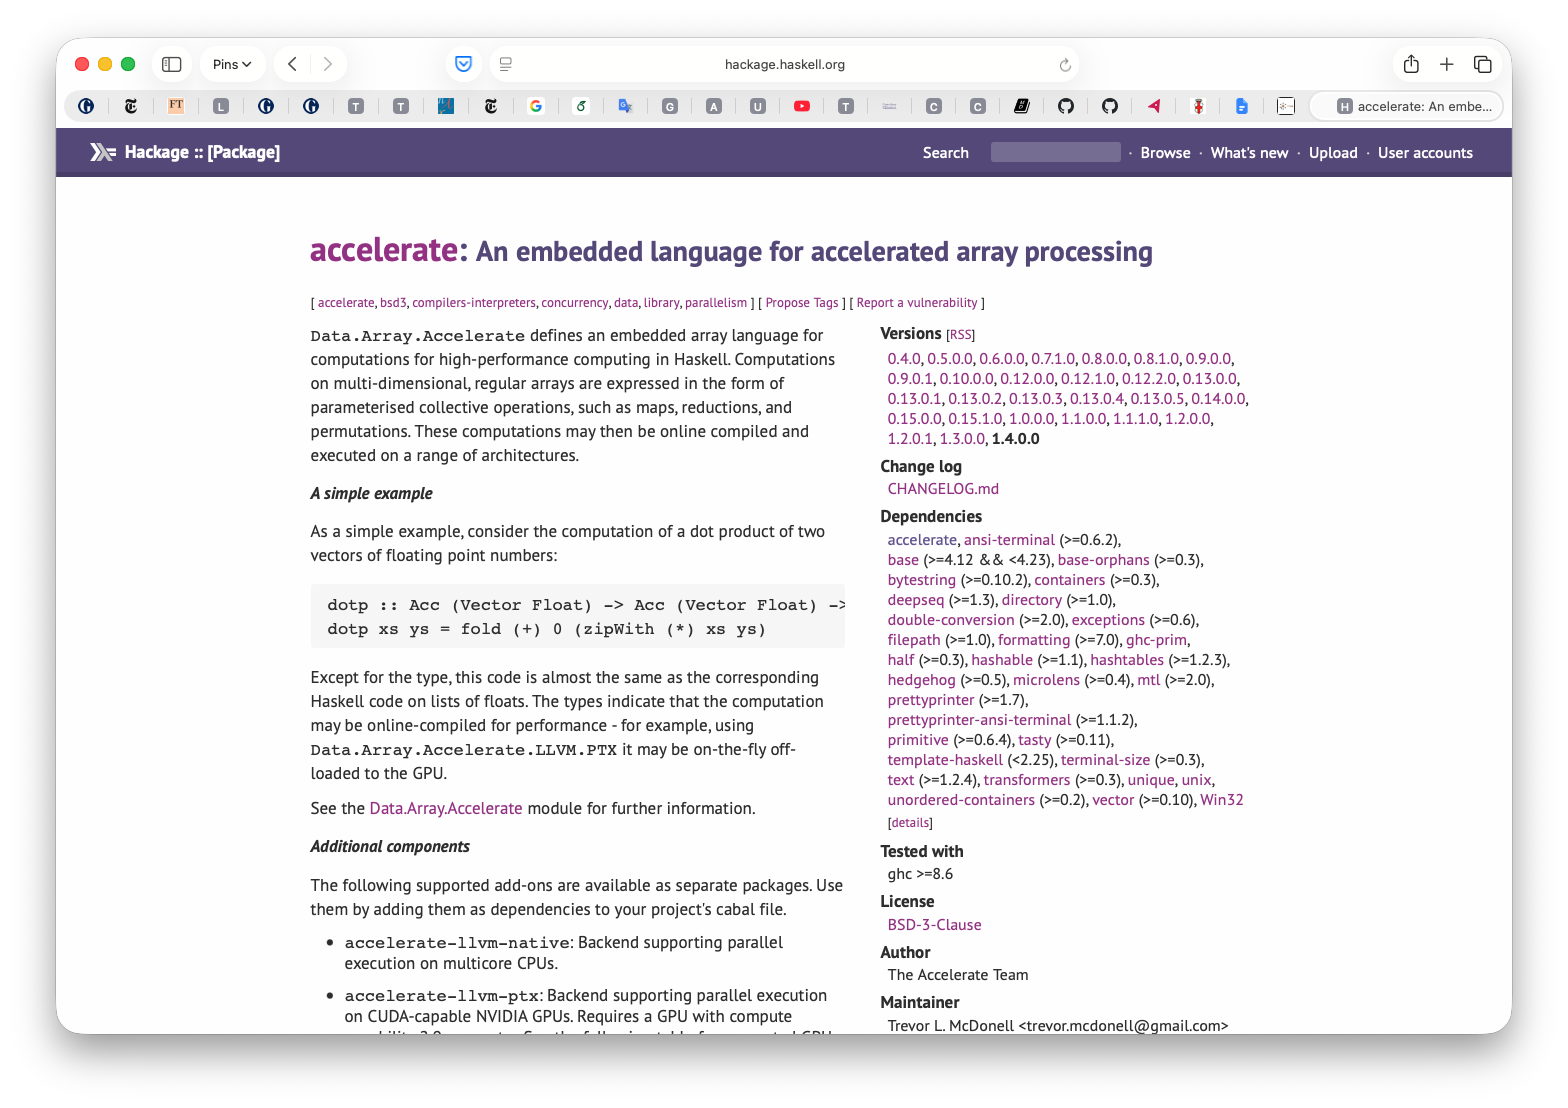
\includegraphics[width=12cm]{Pictures/HackagePic.png}
\end{center} 
\caption{The HackageDB description of the \texttt{accelerate} package}
\label{HackagePic}
\end{figure}

\begin{figure}[t] 
\begin{center}
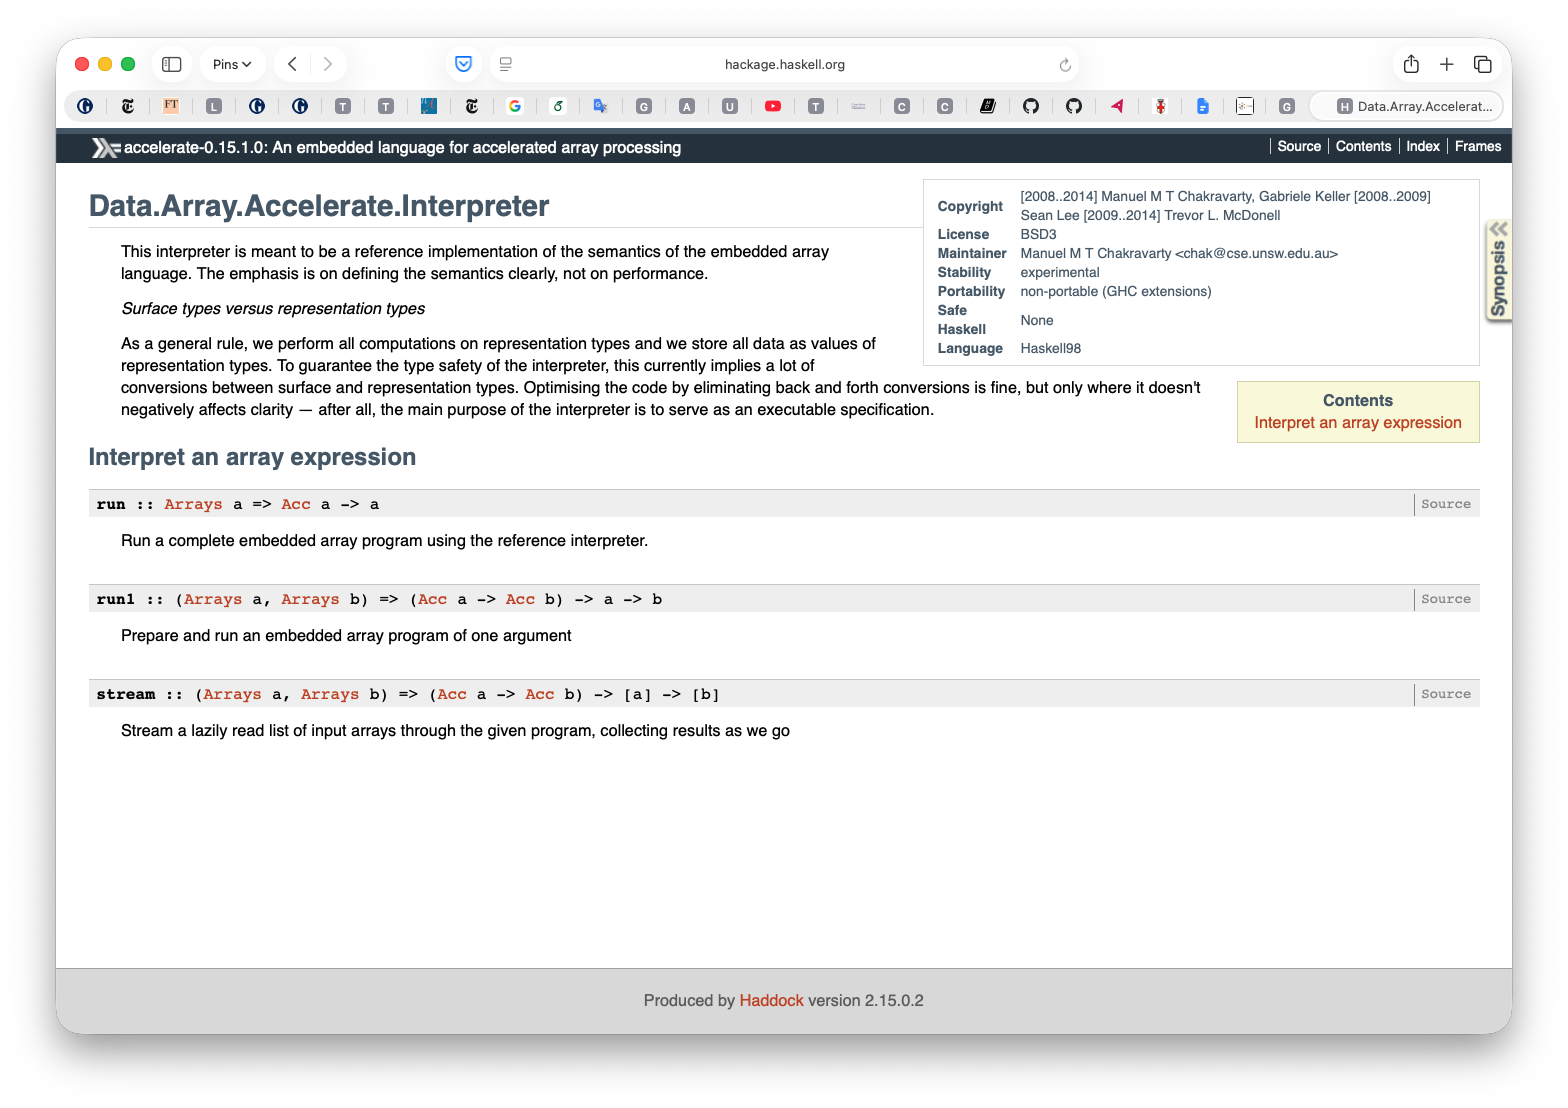
\includegraphics[width=12cm]{Pictures/HaddockPic.png}
\end{center} 
\caption{Haddock documentation for the \texttt{accelerate} package}
\label{Haddock}
\end{figure}


\begin{figure}[t] 
\begin{center}
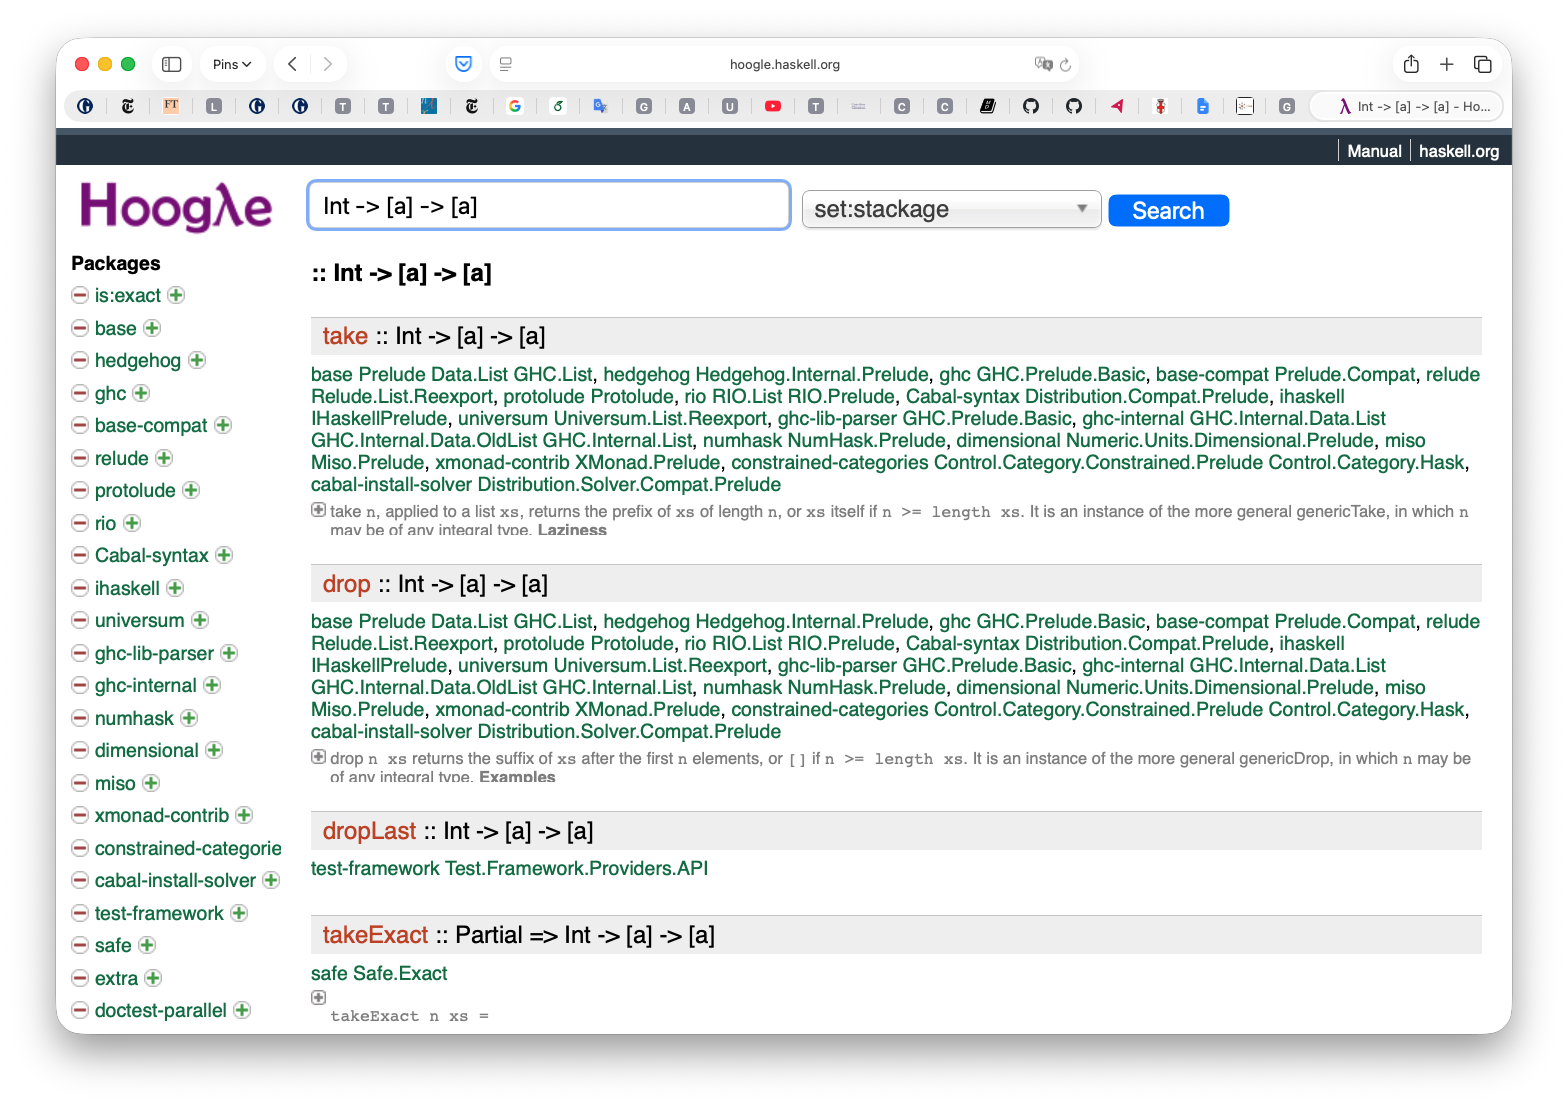
\includegraphics[width=12cm]{Pictures/Hoogle.png}
\end{center} 
\caption{Hoogle in action}
\label{Hoogle}
\end{figure}


\begin{description}
\item[System documentation]\index{documentation!system}
Once GHC is installed via GHCup\index{GHCup}, documentation for the compiler and the libraries that ship with it is also installed locally; GHCup's own documentation, \url{https://www.haskell.org/ghcup/}, explains where to find it on your platform. In practice, though, most readers find it quicker simply to use the online, Hackage-hosted documentation described below, which is always up to date and identical in content.
\item[Libraries]\index{documentation!libraries}
Haddock documentation for the libraries that ship with GHC -- \texttt{base}, \texttt{containers}, \texttt{bytestring} and so on -- is hosted on Hackage alongside everything else; see \textbf{Hackage}, below.
\item[Prelude]\index{documentation!prelude}
In particular, documentation for the \texttt{Prelude}, including descriptions of and examples for many of the functions, is part of the documentation for the \texttt{base} package, and is available directly at \url{https://hackage.haskell.org/package/base/docs/Prelude.html}, which always points to the documentation for whichever version of \texttt{base} ships with the current release of GHC.
\item[Hackage]\index{documentation!Hackage}
Haddock documentation is available for the great majority of packages on Hackage. This is accessible from \url{https://hackage.haskell.org/package/}, which is listed by category, but also searchable. A typical package page is shown in Figure \ref{HackagePic}: documentation for the modules making up the package is linked from the list of modules below the \textbf{Modules} header, towards the bottom of the page; an example is shown in Figure \ref{Haddock}.
\item[Hoogle search]\label{hoogle}\index{documentation!Hoogle}\index{Hoogle}
Hoogle allows you to search many of the standard and Hackage libraries: what is cool about Hoogle is that you can \textbf{search by type} as well as by name. Narrowing down a search by type can lead you very quickly to your answer, or at least eliminate a lot of ``noise'' in a search: \url{https://hoogle.haskell.org/}.
See Figure \ref{Hoogle} for example results. Be aware, though, that Hoogle doesn't cover every package on Hackage. A general web search -- even using a type signature as the search text -- is also often surprisingly effective.
\item[GHCi]\index{documentation!GHCi}\index{GHCi!documentation}
Once you have asked to \texttt{import} a module (\texttt{Foo}, say) into GHCi you can then find out the types of all its exported functions using the GHCi command
\begin{alltt}
:browse Foo
\end{alltt}
Information about a particular function (\texttt{foo}, say) which is in a module loaded in GHCi is given using the command
\begin{alltt} 
:info foo
\end{alltt}
\item[Online resources]
You can go online to ask questions. The Haskell Discourse, \url{https://discourse.haskell.org}, is now the liveliest general home for Haskell discussion and questions; the Haskell Cafe mailing list, \texttt{haskell-cafe@haskell.org}, IRC channels and Stack Overflow's \texttt{haskell} tag remain active too. Links to all of these can be found in the \textbf{Community} section of the Haskell website, \url{https://www.haskell.org}.
\item[Online texts]
Finally, you can find a number of texts online, including the community-maintained continuation of \emph{Learn You a Haskell for Great Good!}, \url{https://learnyouahaskell.github.io/}, and the \emph{Haskell wikibook}, \url{https://en.wikibooks.org/wiki/Haskell}.
\end{description}

\index{libraries, finding your way around|)}





\section{The \texttt{Picture} example: implementation}
\markright{The \texttt{\runinghead  Picture} example: implementation}
\label{picturesAgain}
\index{pictures|(}
\minx{Picture}

In this section we revisit the \texttt{Picture} example, first
introduced in Chapter \ref{intro} and re-examined in Section
\ref{picModuleEx}. What we do here is to look at how to implement
some of the operations over the \texttt{Picture} type, now that we know about list comprehensions and the list functions in the prelude. We also look at how to write more QuickCheck properties for the \texttt{Picture} functions.
\begin{alltt}
type Picture = [[Char]]
\end{alltt}
Some of the operations are defined as library functions. To flip a
picture in a horizontal mirror, we simply have to reverse the order of
the lines of the picture:
\begin{alltt}
flipH :: Picture -> Picture
flipH = reverse\minx{flipH}
\end{alltt}
and to place one picture above another it is sufficient to join the two lists of
lines together:
\begin{alltt}
above :: Picture -> Picture -> Picture
above = (++)\minx{above}
\end{alltt}
where we have enclosed the operator \texttt{++} in parentheses to make it 
a (prefix) function.

How do we flip a picture in a vertical mirror? We have to reverse each
of the lines, that is we have to transform each member of a list in some
way. This is one of the features of a list comprehension, so we can say
\begin{alltt}\index{list comprehensions}\minx{flipV}
flipV :: Picture -> Picture
flipV pic 
  = [ reverse line | line <- pic ]
\end{alltt}
and we can read off from this program its intended effect:
\begin{quote}
``\texttt{reverse} every \texttt{line} in the \texttt{pic}''.
\end{quote}
This is an example of the general operation of applying a function \texttt{f} to every 
element of a list \texttt{xs}, given by the list comprehension
\begin{alltt}
[ f x | x <- xs ]
\end{alltt}
We shall see that this operation is itself a higher-order function in
Chapter \ref{patternsGen} below.

Next we explore how to place two pictures side by side. What we want to
do is to join up the corresponding lines of the two pictures, as
illustrated on page \pageref{beside}. How can we accomplish this? We
can see this as like \texttt{flipV}, in that we want to do something to
every pair of lines -- namely join them with \texttt{++} -- 
but we need to associate corresponding lines before
we do this. That is exactly the purpose of the prelude
function \texttt{zip},\minx{zip} which takes two lists and
pairs corresponding elements, and so we can
say
\begin{alltt}\minx{beside}
beside :: Picture -> Picture -> Picture
beside picL picR
  = [ lineL ++ lineR | (lineL,lineR) <- zip picL picR ]
\end{alltt}
The effect of \texttt{zip} is to chop the list of pairs to the shorter
of the two inputs, and so \texttt{beside} will clip the bottom lines
off whichever picture is the longer; if they are the same length, then
there is no clipping. We can also use the higher-order \texttt{zipWith}
to define \texttt{beside}; we revisit this in Chapter~9.

In our pictures, white is represented by the dot `\texttt{.}' and black
by the hash symbol `\texttt{\#}'. To invert the colour of a single
character we define
\begin{alltt}\minx{invertChar}
invertChar :: Char -> Char
invertChar ch 
  = if ch=='.' then '\#' else '.'
\end{alltt}
The characters `\texttt{.}' and `\texttt{\#}' are swapped by this
definition (and any other character is transformed into `\texttt{.}',
too).
Now, how do we invert the colours in a whole picture? We need to invert
each character in a line, using  
\begin{alltt}\minx{invertLine}
invertLine :: [Char] -> [Char]
invertLine line 
  = [ invertChar ch | ch <- line ]
\end{alltt}
and we want to apply this to all the lines in the picture
\begin{alltt}\minx{invertColour}
invertColour :: Picture -> Picture
invertColour pic 
  = [ invertLine line | line <- pic ]
\end{alltt}
We could if we wish write this as a single definition, thus
\begin{alltt}
invertColour :: Picture -> Picture
invertColour pic 
  = [ [ invertChar ch | ch <- line ] | line <- pic ]
\end{alltt}
but our use of the auxiliary function \texttt{invertLine} makes the
previous
definition more readable.

In the next section we extend our model of pictures to give them a position as well
as some pictorial content.


\subsection*{Tests and properties}

We first discussed writing properties for the functions over pictures in Section \ref{pictureProps}; it's time to look at this again. In that section we looked at properties  of \texttt{flipH} and \texttt{flipV}, separately and together. Here we look at how these functions interact with \texttt{above} and \texttt{beside}, and we look at other properties in the exercises.\index{QuickCheck!pictures}

What happens if we flip \texttt{pic1 `above` pic2} in a vertical mirror? The result is the same as flipping the two pictures separately before putting them together. We can write this as a property
\begin{alltt}\minx{prop\_AboveFlipV}
prop_AboveFlipV :: Picture -> Picture -> Bool

prop_AboveFlipV pic1 pic2 = 
    flipV (pic1 `above` pic2) == (flipV pic1) `above` (flipV pic2) 
\end{alltt}
and test it by typing
\begin{alltt}
quickCheck prop_AboveFlipV
\end{alltt}
(ensuring that the module \texttt{Test.QuickCheck} is loaded.) Similarly we can write the property for \texttt{flipH}:
\begin{alltt}\minx{prop\_AboveFlipH}
prop_AboveFlipH :: Picture -> Picture -> Bool

prop_AboveFlipH pic1 pic2 = 
    flipH (pic1 `above` pic2) == (flipH pic1) `above` (flipH pic2) 
\end{alltt}
but this fails: why? Can you correct the property? Remember that \texttt{flipH} means that we're flipping the picture in a \emph{horizontal} mirror.

In Section \ref{localDefs} we put together four pictures as \texttt{fourPics}. We chose to do this by putting one picture beside another using \texttt{beside}: we could also have done this by putting one picture \texttt{above} another, and we could expect that this gives the same result, as expressed in the property
\begin{alltt}
propAboveBeside :: Picture -> Picture ->  Picture -> Picture -> Bool

propAboveBeside nw ne sw se =
  (nw `beside` ne) `above` (sw `beside` se) 
  == 
  (nw `above` sw) `beside` (ne `above` se) 
\end{alltt}
If we test this, then it fails. Why? Remember that we're using the built-in facilities of QuickCheck to generate \emph{random} values from \texttt{[String]}. If we look at a sample of the data,\footnote{We do this using\ \ \texttt{sample (arbitrary ::\ Gen\  [String]).}} the results look like this:
\begin{alltt}
[]
["a1","\bs{}EOT"]
[]
["","p\bs{}DC3=","\bs{}229\bs{}a\bs{}183","\bs{}218\bs{}SOH\bs{}194",""]
["g\}","P","_y","\bs{}169\bs{}131\bs{}FS\bs{}t","U\bs{}nl",":YicLX\bs{}194\bs{}198","\bs{}t3"] 
 \ldots
\end{alltt}
The elements are random, the pictures are generally not rectangular -- because within each list the strings are of different length -- it is also very likely that four of these chosen randomly will not have the right dimensions to be put together using \texttt{beside} and \texttt{above}. We'll see in Section \ref{qcGens} how to define random \emph{generators} of data for ourselves, and we'll see there how to generate `sensible' random pictures, built up from \texttt{'.'} and \texttt{'\#'} in rectangular patterns, and indeed to generate sets of pictures containing random data but all of the same size.

In the meantime we can say that we only want to check a property when the generated data  satisfy some conditions: let's take a look at an example.
\begin{alltt}
propAboveBeside3Correct :: Picture -> Picture -> Property

propAboveBeside3Correct w e =
  (rectangular w && rectangular e && height w == height e) 
  ==>
     (w `beside` e) `above` (w `beside` e) 
         == 
     (w `above` w) `beside` (e `above` e) 
\end{alltt}
In writing this property we have used \texttt{==>} which we can read as `implies'. 
The property following the \texttt{==>} is only checked when the \texttt{Bool}ean \emph{condition} before the arrow is true. Without the condition the property fails: try it out! 









\begin{exercises}


\item
Define a function
\begin{alltt}
superimposeChar :: Char -> Char -> Char
\end{alltt}
so that the superimposition of `\texttt{.}' with itself gives
`\texttt{.}' while any other combination of characters gives
`\texttt{\#}'.

\item
Define a function
\begin{alltt}
superimposeLine :: [Char] -> [Char] -> [Char]
\end{alltt}
which takes two lines -- which you can assume are of the same length --
and superimposes their corresponding characters using \texttt{superimposeChar}, so that, for example,
\begin{alltt}
superimposeLine ".##." ".#.#" = ".###"
\end{alltt}
You may want to use \texttt{zip} in your solution.

\item
In a similar way to \texttt{superimposeLine},
define the function
\begin{alltt}\minx{superimpose}
superimpose :: Picture -> Picture -> Picture
\end{alltt}
which superimposes two pictures, which you may assume have the same
dimensions. 

\item
Using the function 
\texttt{putStr ::\ String -> IO ()}
and any other functions you might need, define the function 
\begin{alltt}\minx{printPicture}
printPicture :: Picture -> IO ()
\end{alltt}
so that the effect of 
\texttt{printPicture [\,".\#\#."\,, ".\#.\#"\,, ".\#\#\#"\,, "\#\#\#\#"\,]}
is that
\begin{alltt}
.##.
.#.#
.###
####
\end{alltt}
is printed at the terminal window. \emph{Hint:} it is enough to transform this list of strings to the single string
\begin{alltt}
".\#\#.\bs{}n.\#.\#\bs{}n.\#\#\#\bs{}n\#\#\#\#\bs{}n"
\end{alltt}
and to pass that to \texttt{putStr}.


\item {[Harder]} 
Define a function
\begin{alltt}
rotate90 :: Picture -> Picture
\end{alltt}\minx{rotate90}
which rotates a picture through $90^\circ$ clockwise. For
instance, the effect of \texttt{rotate90} on the picture in the previous exercise
would be to give
\begin{alltt}
#...
####
##.#
###.
\end{alltt} 
Hint: you need to make a line of the new picture by picking out the
\texttt{i}th elements in each of the lines of the original picture, reflected 
in a horizontal mirror. 

\item
Using \texttt{rotate90} or otherwise, define a function which rotates a picture through
$90^\circ$ {\em anti}clockwise.

\item
{[Harder]} Define the function
\begin{alltt}\index{scale@\texttt{scale}}
scale :: Picture -> Int -> Picture
\end{alltt}
which scales the input picture by the integer provided as the second
argument. For instance, if \texttt{exPic} is the picture
\begin{alltt}
#.#
..#
\end{alltt}
then the result of \texttt{scale exPic 2} should be
\begin{alltt}
##..##
##..##
....##
....##
\end{alltt}
In the case of a zero or negative scale factor, you should
return an empty picture.


\item
Correct the property \texttt{prop\_AboveFlipH} given earlier.

\item
Define properties which describe how \texttt{beside} interacts with \texttt{flipH} and \texttt{flipV}.

\item
One property we can show holds is that if we take the same picture and put four copies of it together using \texttt{beside} and \texttt{above} in the two different ways, then the results are the same. Express this as a quick check property.

\item
You can test your implementation of \texttt{rotate90} using QuickCheck. Can you think of properties which only use \texttt{rotate90} and others that use \texttt{rotate}? You may want to impose a condition that any picture involved is rectangular: the function is given in the program code for this chapter.

\item
What property would you expect \texttt{invertColour} to have? Can you be sure that this will hold for randomly generated data?

\item {[Harder]}
Write the analogue of \texttt{propAboveBeside3Correct} where two pictures are again used, but with two the same at the top (call them \texttt{n}) and two the same at the bottom (\texttt{s}, say). Do you need the condition in this case?







\end{exercises}
 




\section{Extended exercise: alternative implementations of pictures}
\label{aliterPictures}
\index{extended exercise!picture implementations|(}


This section looks again at the pictures example, and explores alternative implementations. First we look at extending the implementation so that two pictures don't have to be of compatible size when joining them together into one. After that we look at various alternative implementations of pictures as lists.

\subsection*{Incompatible combinations}

In earlier discussions of the \texttt{Picture} type, we have made the assumption that binary functions like \texttt{above} have been called on arguments of compatible size: in the case of \texttt{above} this would mean that the \emph{width} of the two arguments was the same. What should be done if this is not the case? 

We could reasonably assume that each picture was \emph{rectangular} and define the functions so that this \emph{invariant} was preserved by the binary functions. In the example of \texttt{above} this requires that pictures can be padded in an appropriate way. Let's take the specific example of 
\begin{alltt}
(horse `beside` horse)
       `above`
horse
\end{alltt}
as shown in Figure \ref{lshapedhorses}.
\begin{figure}[t]
\begin{center}
\begin{alltt}
.......##..........##...
.....##..#.......##..#..
...##.....#....##.....#.
..#.......#...#.......#.
..#...#...#...#...#...#.
..#...###.#...#...###.#.
.#....#..##..#....#..##.
..#...#.......#...#.....
...#...#.......#...#....
....#..#........#..#....
.....#.#.........#.#....
......##..........##....
.......##...
.....##..#..
...##.....#.
..#.......#.
..#...#...#.
..#...###.#.
.#....#..##.
..#...#.....
...#...#....
....#..#....
.....#.#....
......##....
\end{alltt}
\end{center}
\caption{`Ragged' picture}
\label{lshapedhorses}
\end{figure}
To preserve the rectangular picture, we need to pad out the lower as shown in Figure \ref{paddedhorses}.
\begin{figure}[t]
\begin{center}
\begin{alltt}
.......##..........##...
.....##..#.......##..#..
...##.....#....##.....#.
..#.......#...#.......#.
..#...#...#...#...#...#.
..#...###.#...#...###.#.
.#....#..##..#....#..##.
..#...#.......#...#.....
...#...#.......#...#....
....#..#........#..#....
.....#.#.........#.#....
......##..........##....
.......##...............
.....##..#..............
...##.....#.............
..#.......#.............
..#...#...#.............
..#...###.#.............
.#....#..##.............
..#...#.................
...#...#................
....#..#................
.....#.#................
......##................
\end{alltt}
\end{center}
\caption{``Padded' picture}
\label{paddedhorses}
\end{figure}

\begin{exercises}

\item
Redefine the functions over pictures to pad pictures in the way just described. One way to solve the problem is to use the function
\begin{alltt}
replicate :: Int -> a -> [a]
\end{alltt}
\texttt{replicate n x} returns a list containing \texttt{n} \texttt{x}s, so \texttt{replicate 3 'g'} is \texttt{"ggg"}.

\item
How would you work with basic pictures that were not rectangular? Define a function which will take a picture - as a list of \texttt{String}s -- and return a rectangular list of strings, padding out each line as necessary. Once you start with rectangular pictures the functions you defined in the first part of this exercise should be enough to preserve them as rectangular.
\end{exercises}

\subsection*{Alternative representations}

In this section we look at a number of different ways that these "low fi" pictures can be represented.


\begin{exercises}


\item
An alternative representation of \texttt{Picture} is the type
\begin{alltt}\index{pictures!alternative representation of}
[[Bool]]
\end{alltt}
where \texttt{True}
and \texttt{False} represent black and white points in a picture. How
would you have to modify the functions working over \texttt{Picture} to
accommodate this change? What are the advantages and disadvantages of
the two representations?


\item
We have represented pictures as a list of rows: how would you redefine the functions working over pictures if they are represented as a \emph{list of columns}. 

\item {[Harder]}
How would you re-implement the function \texttt{printPicture}, defined in the solution to exercise 6.7, so that it works over this column-based representation?

\item
It would be possible to represent a \texttt{Picture} as \emph{a single list of characters}, with \texttt{'\bs{}n'} terminating each line of the picture, as in
\begin{alltt}
".\#\#.\bs{}n.\#.\#\bs{}n.\#\#\#\bs{}n\#\#\#\#\bs{}n"
\end{alltt}
How would you redefine the picture manipulating functions over this representation? Which functions become easier to define? Which more difficult?

\end{exercises}

\subsection*{Run-length encoding}\index{run-length encoding}

A more compact representation is given by run-length encoding of Pictures, which will code a repeated character \emph{run} like \texttt{"\#\#\#"} as a pair, \texttt{(3,'\#')}, and a picture is represented as a member of \texttt{[[(Int,Char)]]}. For example, the picture
\begin{alltt}
.##.
.#.#
.###
####
\end{alltt}
is represented like this
\begin{alltt}
[ [(1,'.'), (2,'#'), (1,'.')],
  [(1,'.'), (1,'#'), (1,'.'), (1,'#')],
  [(1,'.'), (3,'#')],
  [(4,'#')] ]
\end{alltt}
using run-length encoding for each row of the picture.

\begin{exercises}

\item
Re-implement the functions over pictures to work with this new representation. In particular, how would you print pictures which were represented in this way?

\item
Is it the case that all your answers to the last question give the most compact representation, so that you don't have adjacent runs of the same character, as in 
\begin{alltt}
[(1,'.'), (2,'.'), (1,'#')]
\end{alltt}
which could be given more compactly as
\begin{alltt}
[(3,'.'), (1,'#')]
\end{alltt}
If this can happen with your functions, how could you change your definitions to avoid it?

\item
Take another look at the QuickCheck properties you wrote to test pictures: rewrite these for your alternative implementations. How many of the properties carry over to the alternative implementations without alteration, and how many have to be modified in some way?

\item {[Harder]}
The run-length encoding above works a line at a time, but it would be possible to give a more compact representation which combines runs in different lines. The earlier example could then be given by 
\begin{alltt}
[(1,'.'), (2,'#'), (2,'.'),
 (1,'#'), (1,'.'), (1,'#'),
 (1,'.'), (7,'#')]
\end{alltt}
This representation loses the length of the rows, so you would have to keep information about the row length in the type too, giving
\begin{alltt}
type Picture = (Int, [(Int,Char)] )
\end{alltt}
as the representation. Re-implement the picture functions to work over this type.

\item {[Harder]}
If you know that only the characters \texttt{'.'} and \texttt{'\#'} are used in a picture, how could you make the representation of the previous question even more compact?

\item {[Harder]}
Define two more representations of pictures yourself, and re-implement the picture functions over these types.



\end{exercises}

\index{extended exercise!picture implementations|)}




\section{Extended exercise: positioned pictures}
\label{posPix}
\index{extended exercise!positioned pictures|(}

The pictures that we have modelled using the type \texttt{Picture} are not
anchored at any particular point in space: 
we can think of them concretely as being on pieces of
paper which can be joined together, superimposed, rotated and so on.

A different model of pictures gives each picture a \texttt{Position}\minx{Position} in
space: we can then think of moving these pictures, of superimposing
two of these pictures to give another picture, and so on.
\begin{figure}[t]
\begin{center}
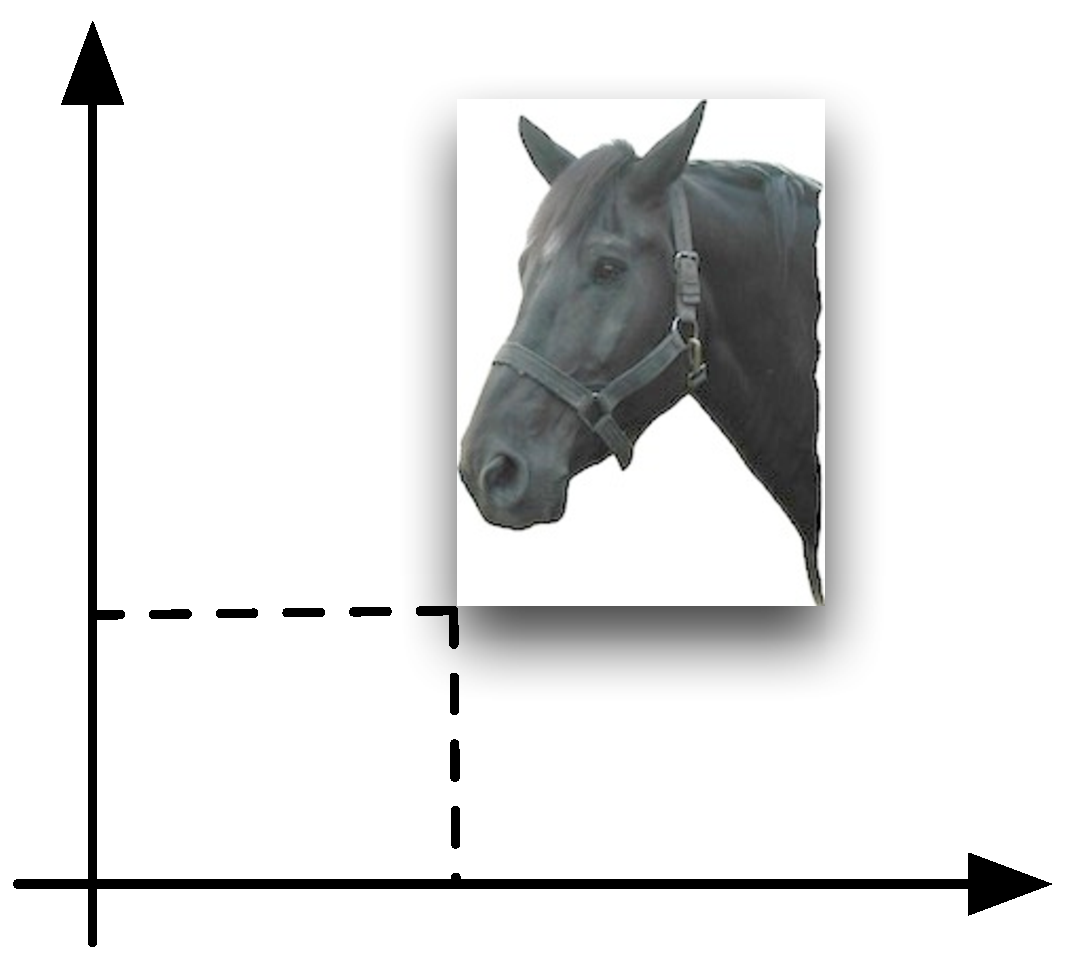
\includegraphics[width=2.5in]{Pictures/horsePos.pdf}
\end{center}
\caption{An example \texttt{Image}.\label{horsePos}}
\end{figure}

\subsection*{Basics}

How can we represent pictures with positions? First we need to
think about how we model positions on an {\em integer\/}
grid. A \texttt{Position} is given by a pair of integers,
\begin{alltt}
type Position = (Int,Int)
\end{alltt}
We will use the term \texttt{Image} for a picture with a position, and
so we define
\begin{alltt}\minx{Image}
type Image = (Picture,Position)
\end{alltt}
An example, in which we position the \texttt{horse} with its bottom
left-hand corner or \textbf{reference point}\index{reference point} at 
position \texttt{(31,23)}, is given in Figure
\ref{horsePos}.

The remainder of this section is a collection of exercises to write functions
which manipulate these \texttt{Images}; you can use any of the list
functions introduced in the previous chapter and also the functions
over \texttt{Picture}
which we have already defined.

\begin{exercises}


\item
Define a function
\begin{alltt}\minx{makeImage}
makeImage :: Picture -> Position -> Image
\end{alltt}
which makes an \texttt{Image}
from a \texttt{Picture} and a \texttt{Position}.

\item
Define a function
\begin{alltt}\minx{changePosition}
changePosition :: Image -> Position -> Image
\end{alltt}
which takes an \texttt{Image}
and returns a new \texttt{Image} whose \texttt{Picture} is unchanged but whose \texttt{Position}
is given by the second argument to \texttt{changePosition}.

\item
Give a definition of the function
\begin{alltt}\minx{moveImage}
moveImage :: Image -> Int -> Int -> Image
\end{alltt}
so that the effect of \texttt{moveImage img xMove yMove} is to move \texttt{img}
by \texttt{xMove} in the horizontal (\texttt{x}) direction and by \texttt{yMove} in
the vertical (\texttt{y}) direction.

\item
Define a function
\begin{alltt}
printImage :: Image -> IO ()
\end{alltt}
whose action is the analogue of \texttt{printPicture} for pictures.

\begin{figure}[t]
\begin{center}
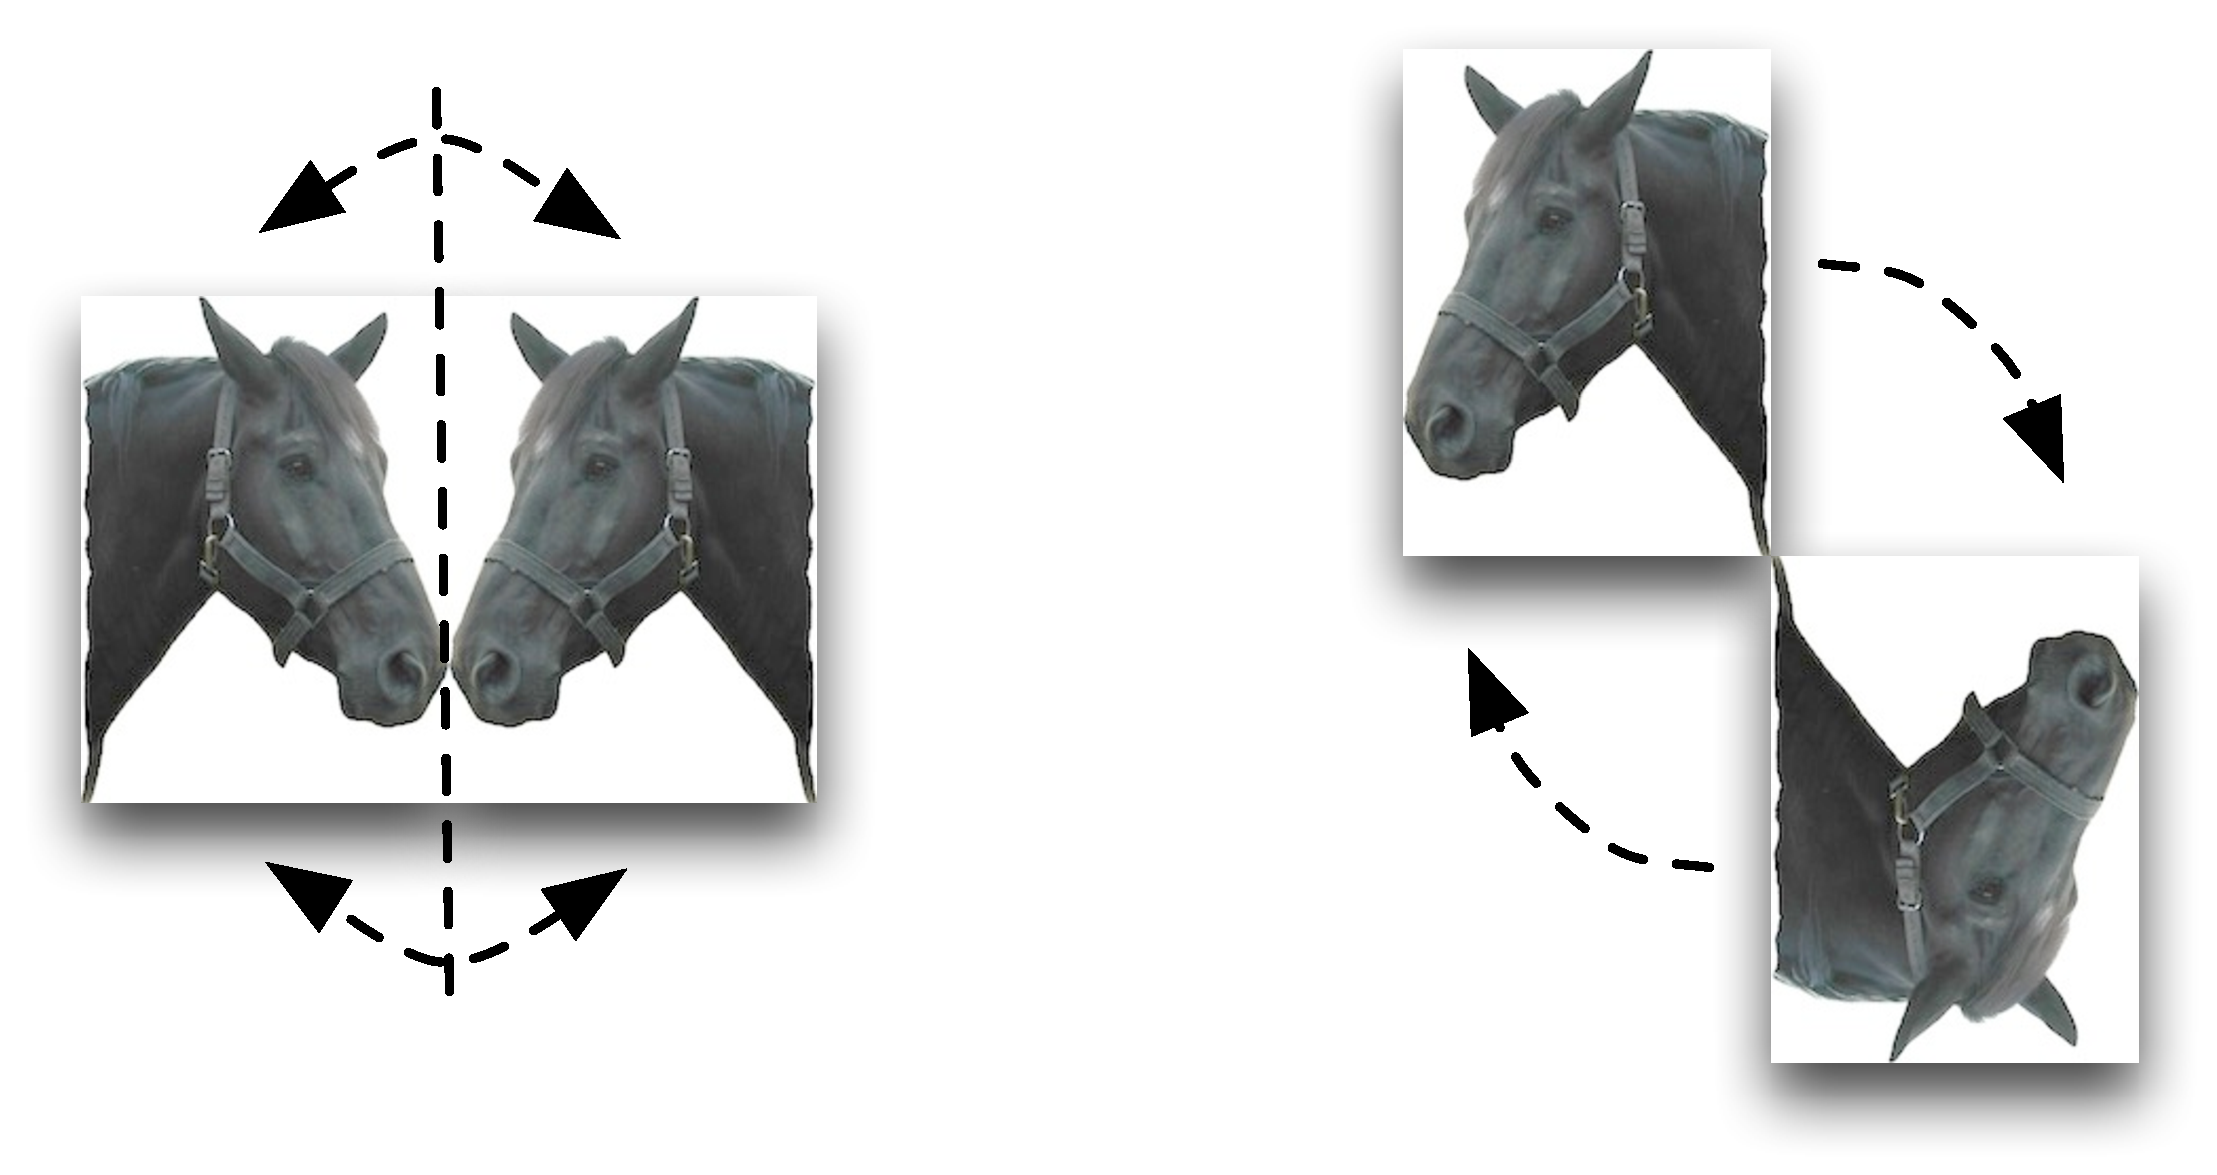
\includegraphics[width=4in]{Pictures/transfPos.pdf}
\end{center}
\caption{The geometrical view of \texttt{flipV} and \texttt{rotate}.}
\label{transfPos}
\end{figure}
\end{exercises}

\subsection*{Transformations}

We can extend the transformations over the type \texttt{Picture}
to the \texttt{Image} type, but we need to think about the effect of
these transformations on the position. One way to lift the
transformations from pictures to images
is simply to say that the pictures stay in the same
position -- we call this the \textbf{naive} view. 


If we think of reflections and rotations going on in space, then the
results are more likely to be as  shown in Figure \ref{transfPos},
where we see that the position of the resulting image has changed. Rotation is
about the reference point, and reflection is in the horizontal or vertical line through
the reference point; in general these operations will change the reference point. We
call this the \textbf{geometrical} view of the transformations. 

\begin{exercises}
\item
Implement for \texttt{Image} the analogues of \texttt{flipH}, \texttt{flipV},
\texttt{rotate} and \texttt{rotate90} under the naive view of how to lift the 
transformations.

\item
Implement for \texttt{Image} the analogues of \texttt{flipH}, \texttt{flipV},
\texttt{rotate} and \texttt{rotate90} under the geometrical view.
\end{exercises}

\subsection*{Superimposition}

When pictures have positions, superimposition can be more complex.
Consider the example illustrated in Figure \ref{superPos};
here we see one way of superimposing the two images is to use
\texttt{Picture} superimposition on two pictures which have first been
`padded out' with white space as shown in the figure. 

\begin{figure}[t]
\begin{center}
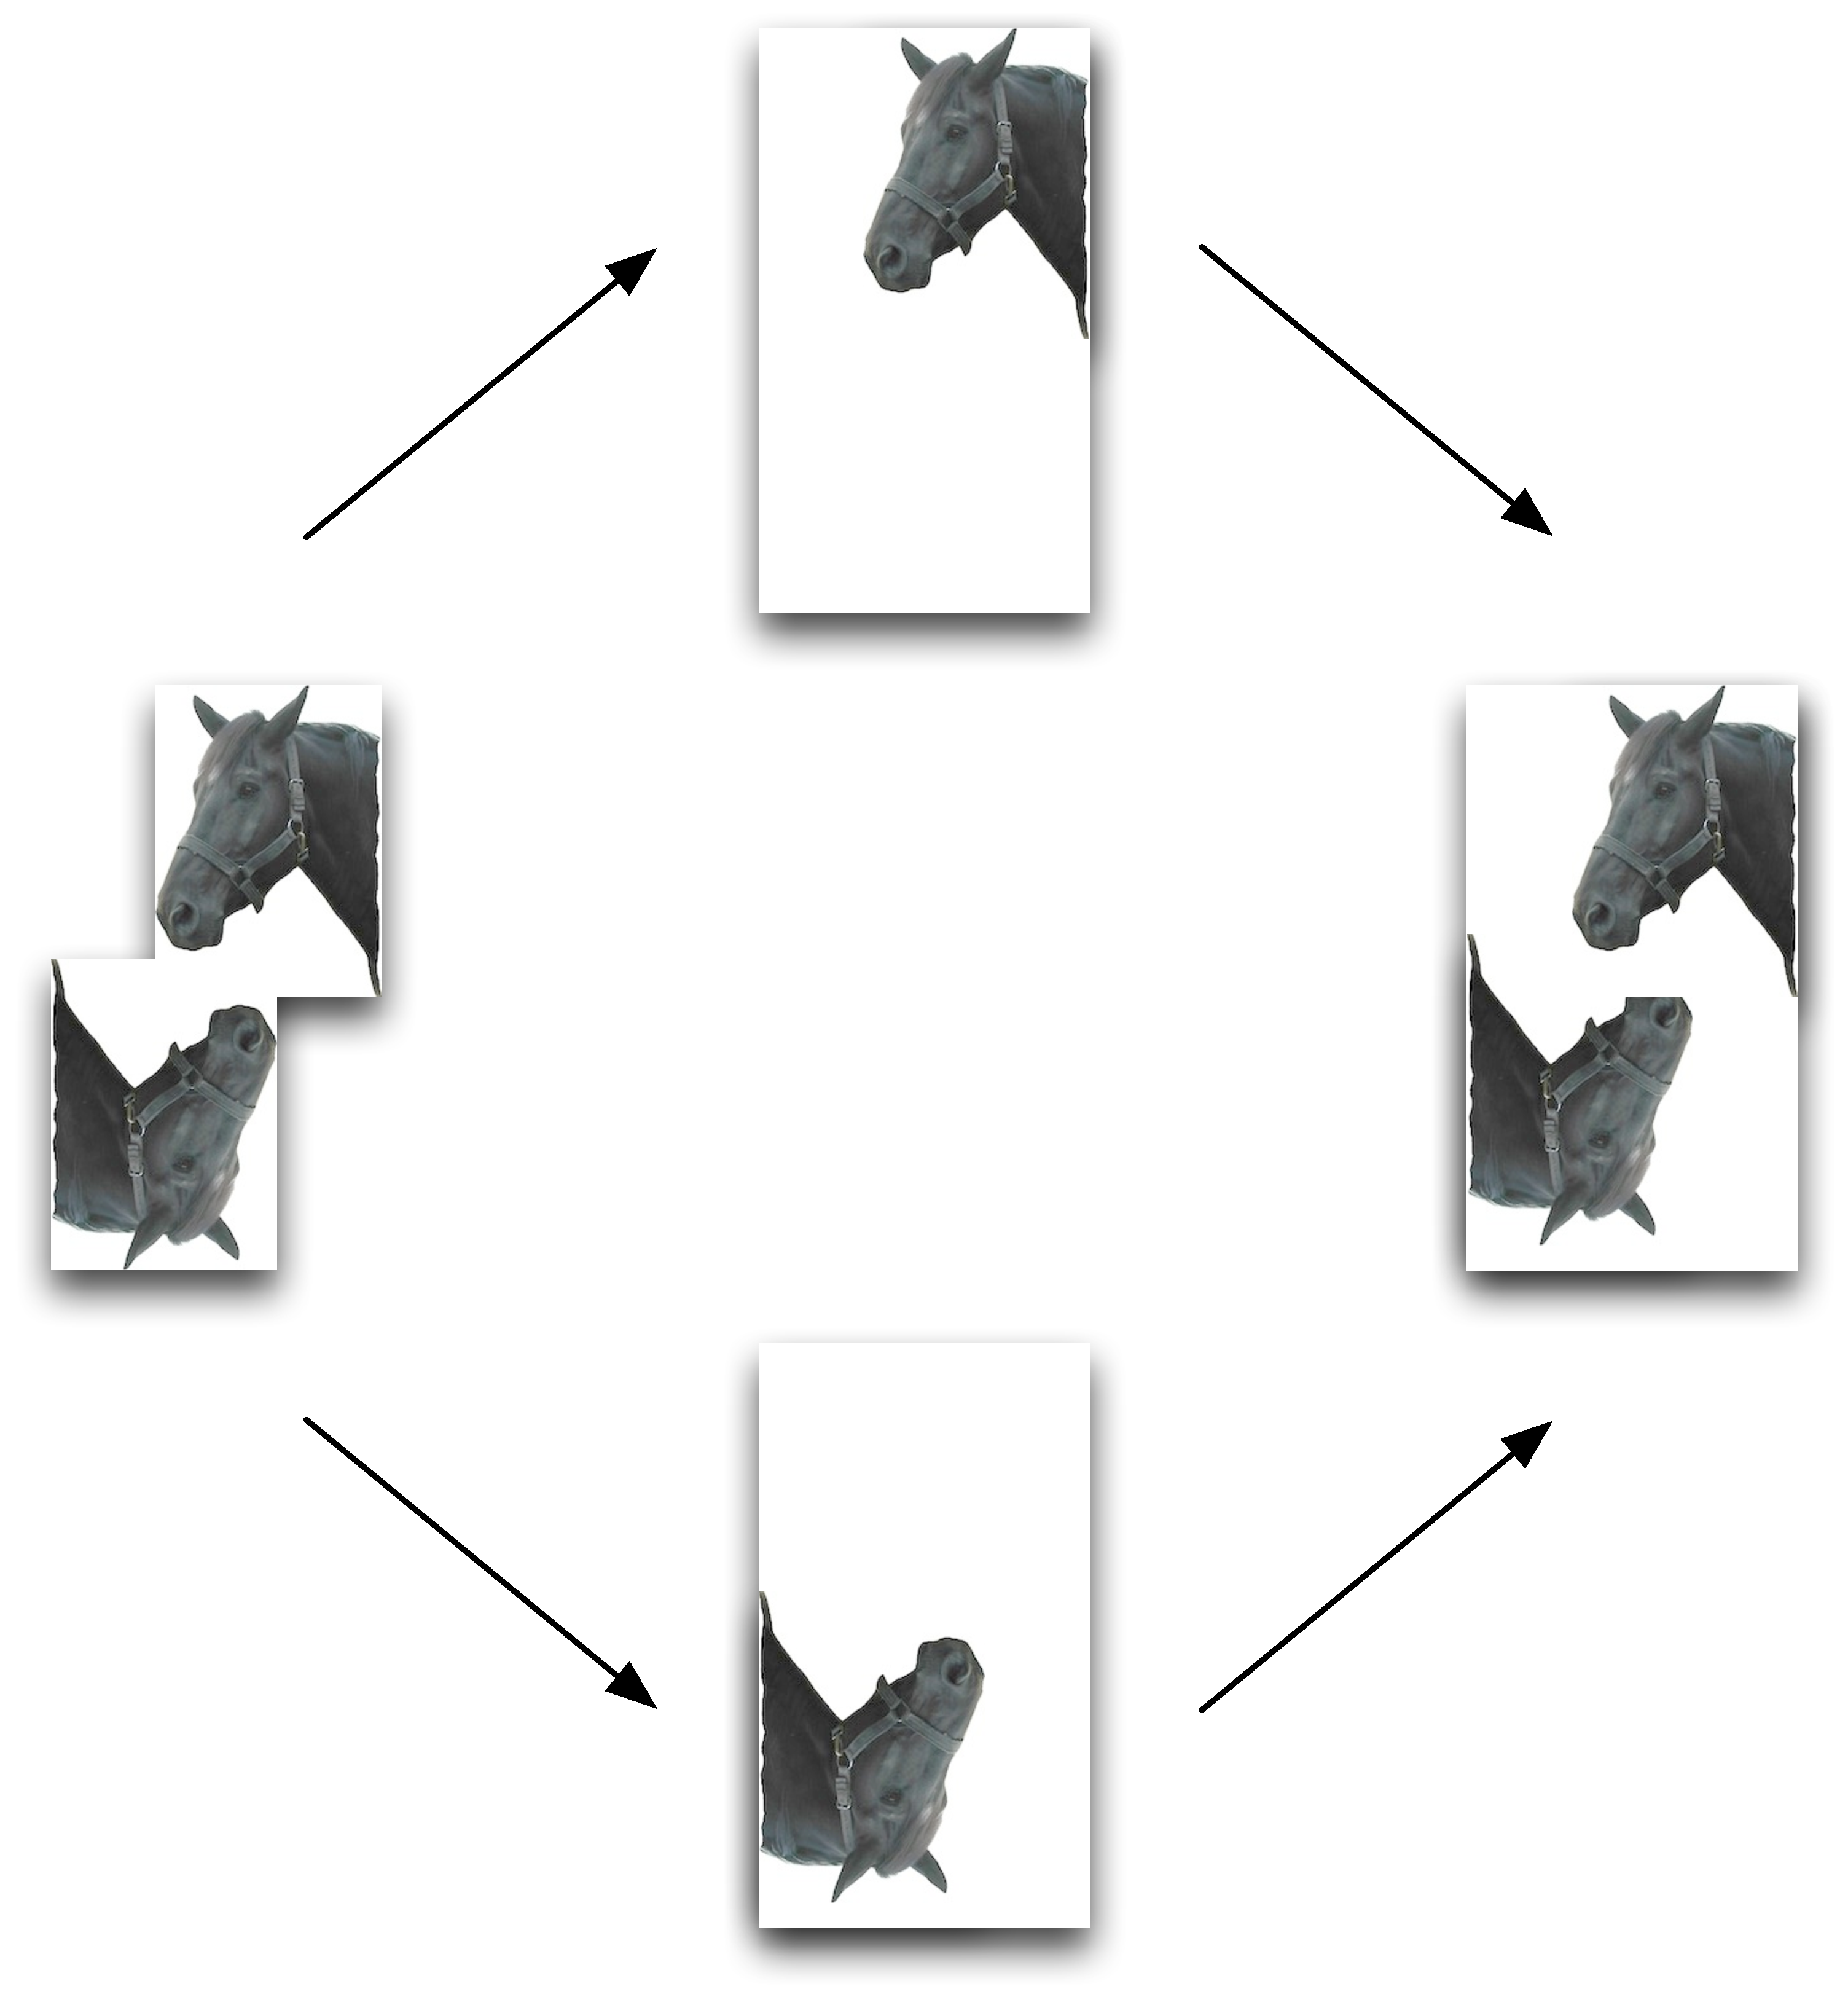
\includegraphics[width=3in]{Pictures/superPos.pdf}
\end{center}
\caption{Superimposing two \texttt{Images}.}
\label{superPos}
\end{figure}


\begin{exercises}


\item
Define functions to `pad out' a \texttt{Picture}
with an amount of white space, as shown in Figure \ref{superPos}.

You will need to think carefully about
the intended effect of the functions before you start to
implement them. You will need to have function parameters for the amount of padding
to the left, right, bottom and top of the image.

Note, in particular, that the \texttt{Position} of an
\texttt{Image} might change as a result of padding.

\item
Using the padding functions, define a superimposition function for
the \texttt{Image} type.

\item
How would you use \texttt{Image} superimposition to give analogues of 
\texttt{above} and \texttt{beside} for \texttt{Images}?

\item 
Define QuickCheck properties to check the implementation of the functions over the \texttt{Image} type. How many carry over from the \texttt{Picture} type, and how many have to be re-defined?

\index{pictures|)}
\index{extended exercise!positioned pictures|)}

\end{exercises}


\section{Extended exercise: supermarket billing}
\label{superBill}
\index{examples!supermarket billing|see{supermarket billing}}
\index{supermarket billing|(}

This collection of exercises looks at supermarket billing.\footnote{I am
grateful to Peter Lindsay {\em et\ al.\ }of the Department of
Computer Science at the University of New South Wales, Australia, for the
inspiration for this example, which was suggested by their lecture
notes.} The idea is to use the
list-manipulating techniques presented in Chapter \ref{tupleList}. In particular
we will be using list comprehensions and also the prelude functions
mentioned there. We will also expect local definitions -- as explained
in Section \ref{localDefs} -- to be used when
appropriate.

\begin{figure}[t]
\begin{alltt}
                          Haskell Stores\index{Haskell Stores@\verb+Haskell Stores+}
                     
                  Dry Sherry, 1lt...........5.40
                  Fish Fingers..............1.21
                  Orange Jelly..............0.56
                  Hula Hoops (Giant)........1.33
                  Unknown Item..............0.00
                  Dry Sherry, 1lt...........5.40
                       
                  Total....................13.90
\end{alltt}
\caption{A supermarket bill}
\label{basicBill}
\end{figure}


\subsection*{The problem}

A scanner at a supermarket checkout will produce from a basket
of shopping a list of bar codes,
like
\begin{alltt}
[1234,4719,3814,1112,1113,1234]
\end{alltt}
which has to be converted to a bill as shown in Figure \ref{basicBill}
We have to decide first how to model the objects involved. Bar codes and
prices (in pence) can be modelled by integers; names of goods by strings. We
say therefore that
\begin{alltt}
type Name    = String
type Price   = Int
type BarCode = Int
\end{alltt}
The conversion will be based on a \textbf{database}\index{database}
which links bar
codes, names and prices. As in the library, we use a list to model the
relationship. 
\begin{alltt}\minx{Database}
type Database = [ (BarCode,Name,Price) ]
\end{alltt}
The example database we use is
\begin{alltt}
codeIndex :: Database
codeIndex = [ (4719, "Fish Fingers" , 121),
              (5643, "Nappies" , 1010),
              (3814, "Orange Jelly", 56),
              (1111, "Hula Hoops", 21),
              (1112, "Hula Hoops (Giant)", 133),
              (1234, "Dry Sherry, 1lt", 540)]
\end{alltt}
The object of the script will be to convert a list of bar codes into a list
of \texttt{(Name,Price)} pairs; this then has to be converted into a string
for printing as above. We make the type definitions
\begin{alltt}
type TillType = [BarCode]
type BillType = [(Name,Price)]
\end{alltt} 
and then we can say that the functions we wish to define are 
\begin{alltt}
makeBill    :: TillType -> BillType\minx{makeBill}
\end{alltt}
which takes a list of bar codes to a list of name/price pairs,
\begin{alltt}
formatBill  :: BillType -> String\minx{formatBill}
\end{alltt}
which takes a list of name/price pairs into a formatted bill, and
\begin{alltt}
produceBill :: TillType -> String\minx{produceBill}
\end{alltt}
which will combine the effects of \texttt{makeBill} and
\texttt{formatBill}, thus
\begin{alltt}
produceBill = formatBill . makeBill
\end{alltt}
The length of a line in the bill is decided to be \texttt{30}. This is made a
constant, thus
\begin{alltt}
lineLength :: Int
lineLength = 30
\end{alltt}
Making \texttt{lineLength} a constant in this way means that to change the
\index{definition!constant!reason for}
length of a line in the bill, only one definition needs to be altered; if
\texttt{30} were used in each of the formatting functions, then each would have
to be modified on changing the line length. 
The rest of the script is developed through the sequences of
exercises which follow. 

\subsection*{Formatting the bill}
 
First we develop the \texttt{formatBill} function from
the bottom up: we design functions to format prices, lines, and the total, and
using these we finally build the \texttt{formatBill} function itself.

\begin{exercises}

\item
Given a number of pence, \texttt{1023} say, the pounds and pence parts are given
by \texttt{1023 `div` 100} and \texttt{1023 `mod` 100}. Using this fact, and the 
\texttt{show} function, define a function
\begin{alltt}
formatPence :: Price -> String
\end{alltt}
so that, for example, \texttt{formatPence 1023 = "10.23"}; you need to be
careful about cases like \texttt{"12.02"}.

\item
Using the \texttt{formatPence} function, define a function
\begin{alltt}
formatLine  :: (Name,Price) -> String
\end{alltt}
which formats a line of a bill, thus
\begin{alltt}
formatLine ("Dry Sherry, 1lt",540) 
               = "Dry Sherry, 1lt...........5.40\bs{n}"
\end{alltt}
Recall that \texttt{'\bs{n}'} is the newline character, 
that \texttt{++} can be used
to join two strings together, and that \texttt{length} will give the length of a
string. You might also find the \texttt{replicate} function useful.

\item
Using the \texttt{formatLine} function, define
\begin{alltt}
formatLines :: [ (Name,Price) ] -> String
\end{alltt}
which applies \texttt{formatLine} to each \texttt{(Name,Price)} pair, and joins the
results together. 

\item
Define a function 
\begin{alltt}
makeTotal :: BillType -> Price
\end{alltt}
which takes a list of \texttt{(Name,Price)} pairs, and gives the total of the
prices. For instance,
\begin{alltt}
makeTotal [(" ... ",540),(" ... ",121)] = 661
\end{alltt}

\item
Define the function
\begin{alltt}
formatTotal :: Price -> String
\end{alltt}
so that, for example,
\begin{alltt}
formatTotal 661 = "\bs{n}Total.....................6.61"
\end{alltt}

\item
Using the functions \texttt{formatLines}, \texttt{makeTotal} and \texttt{formatTotal},
define 
\begin{alltt}
formatBill :: BillType -> String\minx{formatBill}
\end{alltt} 
so that on the input
\begin{alltt}
[("Dry Sherry, 1lt",540),("Fish Fingers",121),
("Orange Jelly",56),("Hula Hoops (Giant)",133),
("Unknown Item",0),("Dry Sherry, 1lt",540)]
\end{alltt}
the example bill at the start of the section is produced.

\end{exercises}
\subsection*{Making the bill: bar codes into names and prices}

Now we have to look
at the database functions which accomplish the conversion of bar codes into 
names and prices.

\begin{exercises}

\item
Define a function
\begin{alltt}
look :: Database -> BarCode -> (Name,Price)
\end{alltt}
which returns the \texttt{(Name,Price)} pair corresponding to the \texttt{BarCode}
in the \texttt{Database}. If the \texttt{BarCode} does not appear in the database,
then the pair \texttt{("Unknown Item", 0)} should be the result.

Hint: using the ideas of the library database you might find that you
are returning a {\em list\/} of \texttt{(Name,Price)}
rather than a single value. You can assume
that each bar code occurs only once in the database, so you can extract
this value by taking the \texttt{head} of such a list {\em if it is non-empty}.

\item
Define a function
\begin{alltt}
lookup :: BarCode -> (Name,Price)
\end{alltt}
which uses \texttt{look} to look up an item in the particular database {\mi
codeIndex}. This function clashes with a function \texttt{lookup}
defined in the prelude; consult page \pageref{redefName} for details of how to
handle this.

\item
Define the function 
\begin{alltt}
makeBill   :: TillType -> BillType\minx{makeBill}
\end{alltt}
which applies \texttt{lookup} to every item in the input list. For instance,
when applied to \texttt{[1234,4719,3814,1112,1113,1234]} the result will be
the list of \texttt{(Name,Price)} pairs given in Exercise 6.25.
Note that \texttt{1113} does not appear in \texttt{codeIndex} and so is converted
to \texttt{("Unknown Item",0)}.

This completes the definition of \texttt{makeBill} and together
with 
\texttt{formatBill} gives the conversion program. 
\end{exercises}

\subsection*{Extending the problem}

We conclude with some further
exercises.

\begin{exercises}
\item
You are asked to add a discount for multiple buys
of sherry: for every two bottles bought, there is a %\pounds 
\texttt{1.00} discount. From the example list of bar codes
\begin{alltt}
[1234,4719,3814,1112,1113,1234]
\end{alltt}
the bill should be as illustrated in 
Figure \ref{newBill}.
\begin{figure}[t]
\begin{alltt}
                          Haskell Stores
                     
                  Dry Sherry, 1lt...........5.40
                  Fish Fingers..............1.21
                  Orange Jelly..............0.56
                  Hula Hoops (Giant)........1.33
                  Unknown Item..............0.00
                  Dry Sherry, 1lt...........5.40
                     
                  Discount..................1.00
                     
                  Total....................12.90
\end{alltt}
\caption{Bills with `multibuy' discounts.}
\label{newBill}
\end{figure}
You will probably find it helpful to define functions
\begin{alltt}
makeDiscount :: BillType -> Price
formatDiscount :: Price -> String
\end{alltt}
which you can use in a redefined
\begin{alltt}
formatBill :: BillType -> String
\end{alltt}

\item
Design functions which update the database of bar codes. You will need a
function to add a \texttt{BarCode} and a \texttt{(Name,Price)} pair to the {\mi
Database}, while at the same time removing any other reference to the bar
code already present in the database.

\item
Re-design your system so that bar codes which do not appear in the database
give no entry in the final bill. There are (at least) two ways of doing this.
\begin{titemize}
\item Keep the function \texttt{makeBill} as it is, and modify the 
formatting functions, or
\item modify the \texttt{makeBill} function to remove the `unknown item' pairs.
\end{titemize}


\item
{[Harder]}
How appropriate would it be to test your supermarket billing system using QuickCheck? Could you check parts of the system using QuickCheck? Could you use it to test the whole system, or could you do both?


\item
{[Project]} Design a script of functions to analyse collections
of sales. Given a list of \texttt{TillType}, produce a table
showing the total sales of each item. You might also analyse
the bills to see which {\em pairs\/} of items are bought
together; this could assist with placing items in the
supermarket.


\index{supermarket billing|)}
\end{exercises}

\section{Extended exercise: cards and card games}
\label{cardGames}
\index{extended exercise!card games|(}

\begin{wrapfigure}[8]{r}{5cm}
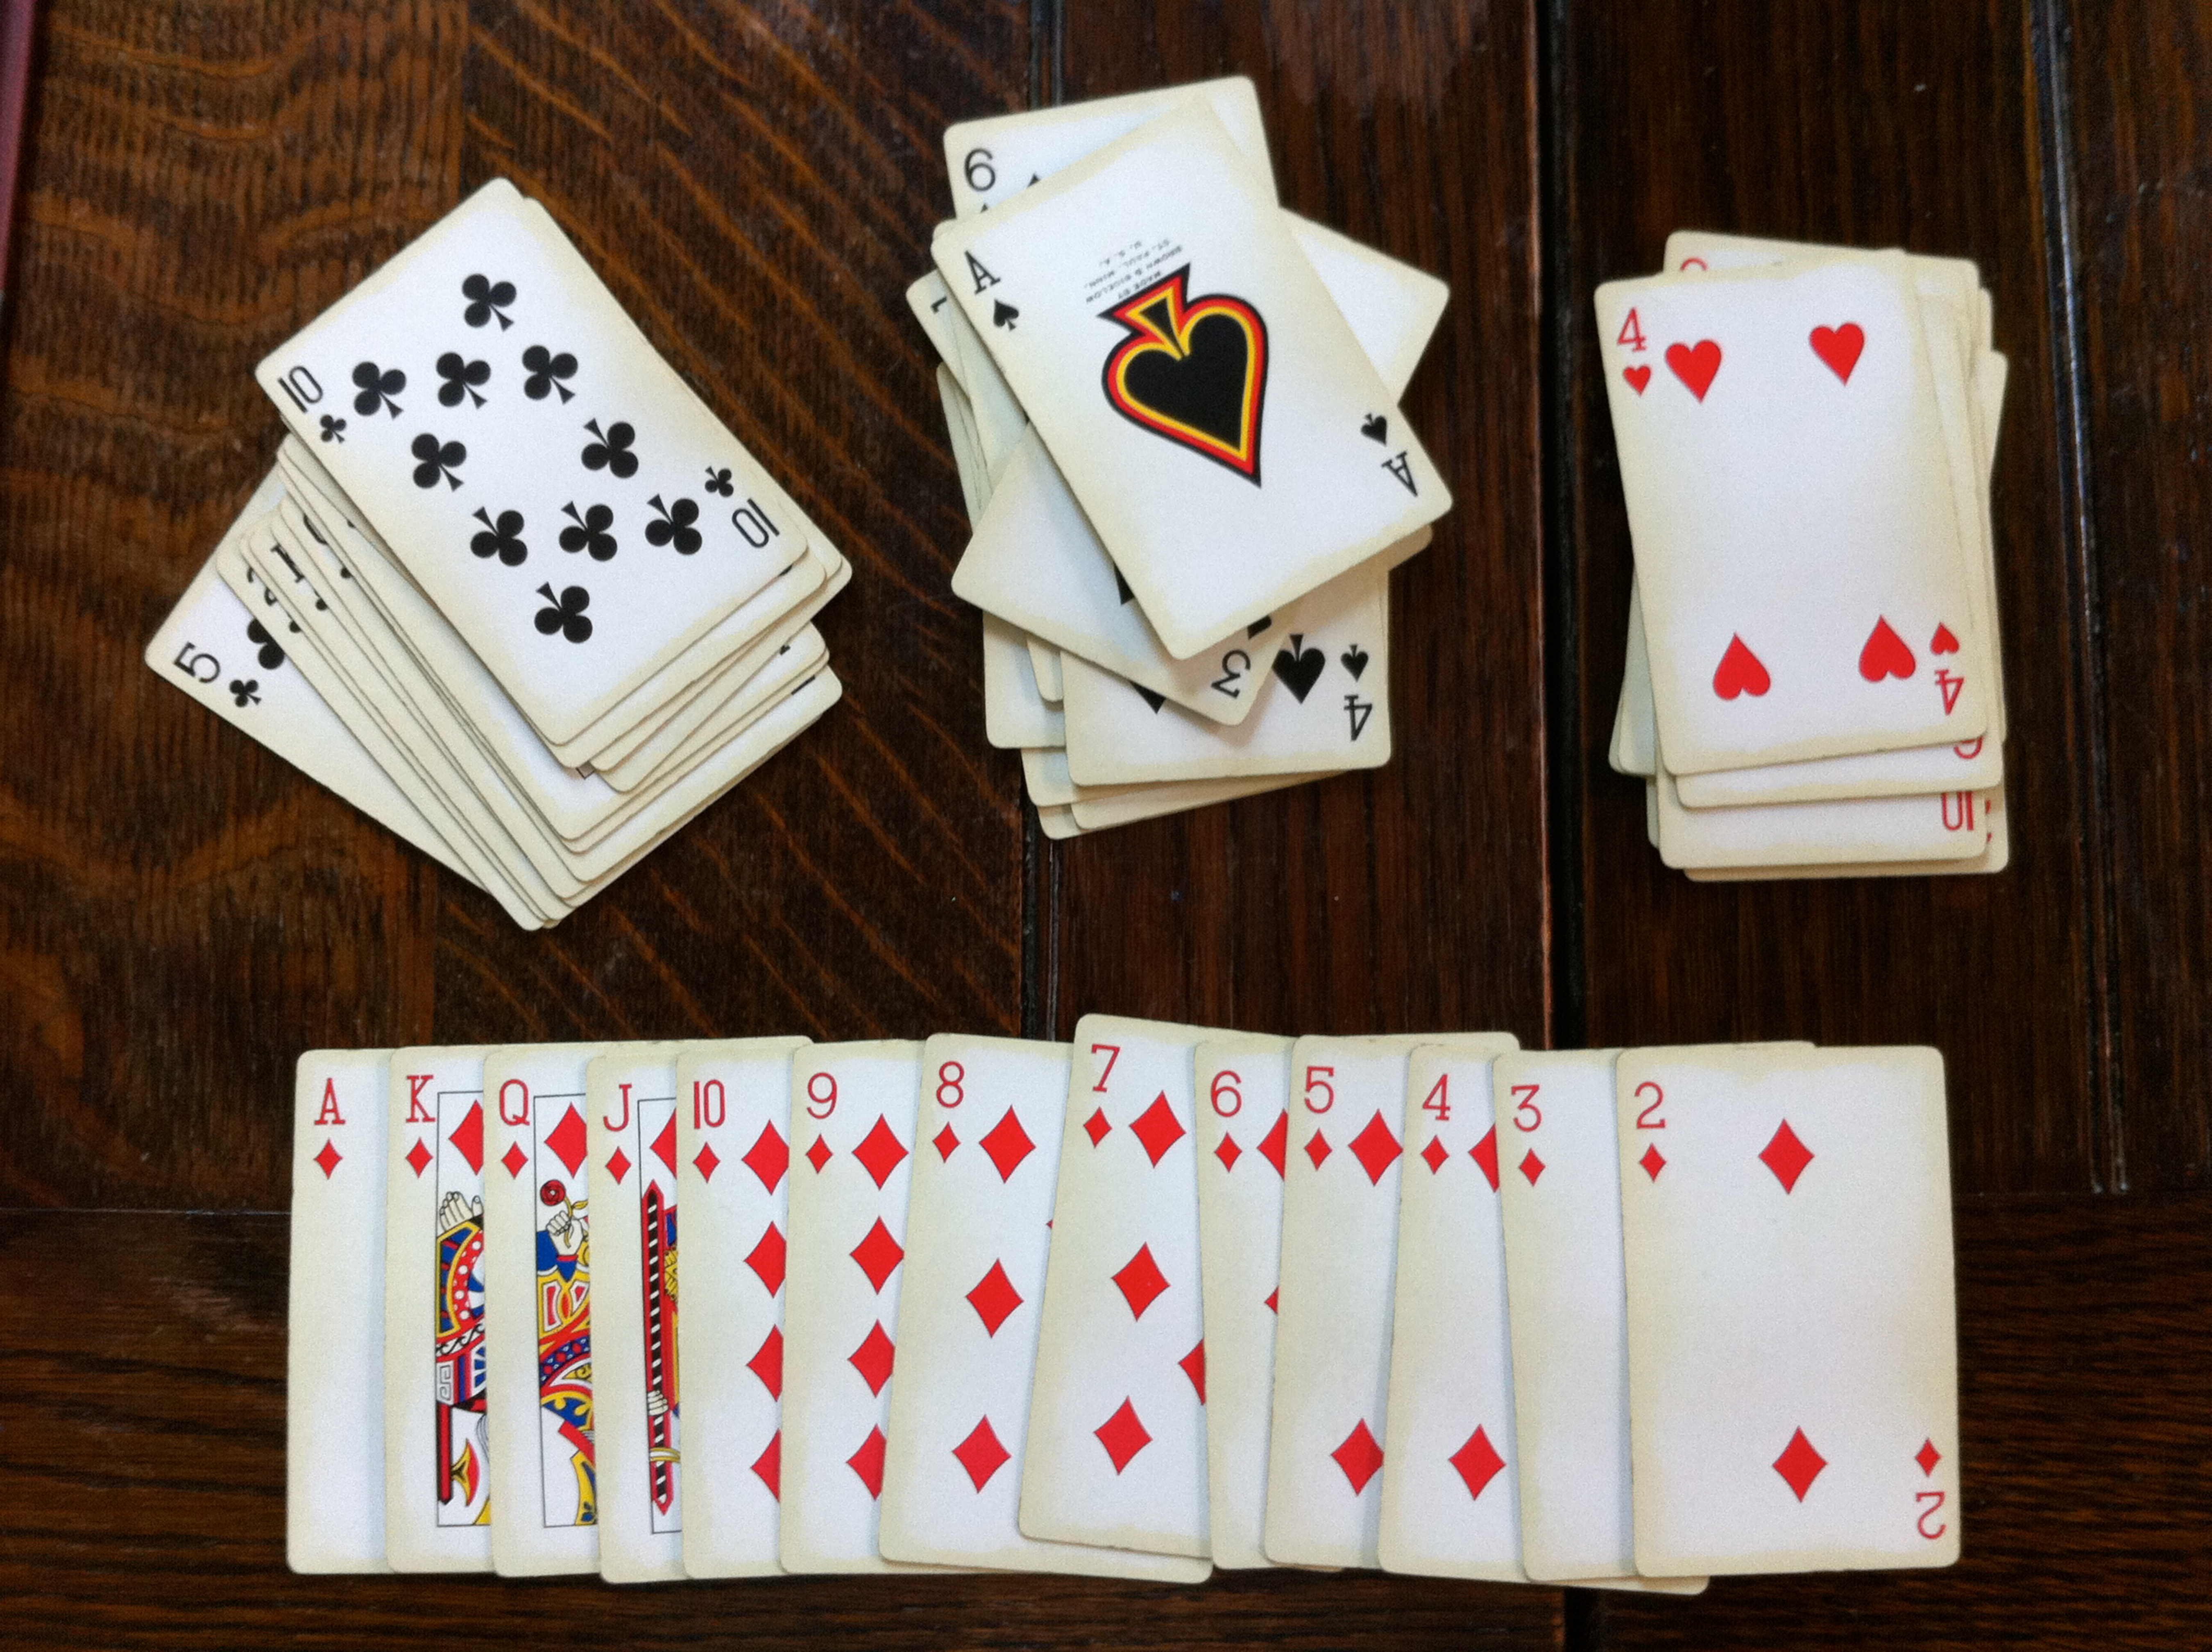
\includegraphics[width=5cm]{Pictures/Cards.pdf}
\end{wrapfigure}
An British deck (or pack) of cards has four suits: spades (\spade), hearts (\heart), diamonds (\dia) and clubs (\club). 

Each suit\index{suit} contains cards 2 to 10, and the court cards, Jack, Queen, King and Ace. The values of the cards increase in the same order, so, for example, a 9 beats a 2, a King beats a 10, and an Ace beats everything (in this discussion we're taking ``Aces high'').

\begin{exercises}

\item
Define a type \texttt{Suit} to represent \emph{suits} and a type \texttt{Value} to represent the \emph{value} of cards. Using these or otherwise, define a type \texttt{Deck} to represent a deck of cards. You may use type synonyms (\texttt{type}) or data type definitions (\texttt{data}), or both. 

\item Try to give a rationale for the choices you have made in answering the previous question: if you can, give alternative definitions which use the other mechanism, and compare your solutions. 

\end{exercises}

\begin{wrapfigure}[7]{r}{2cm}
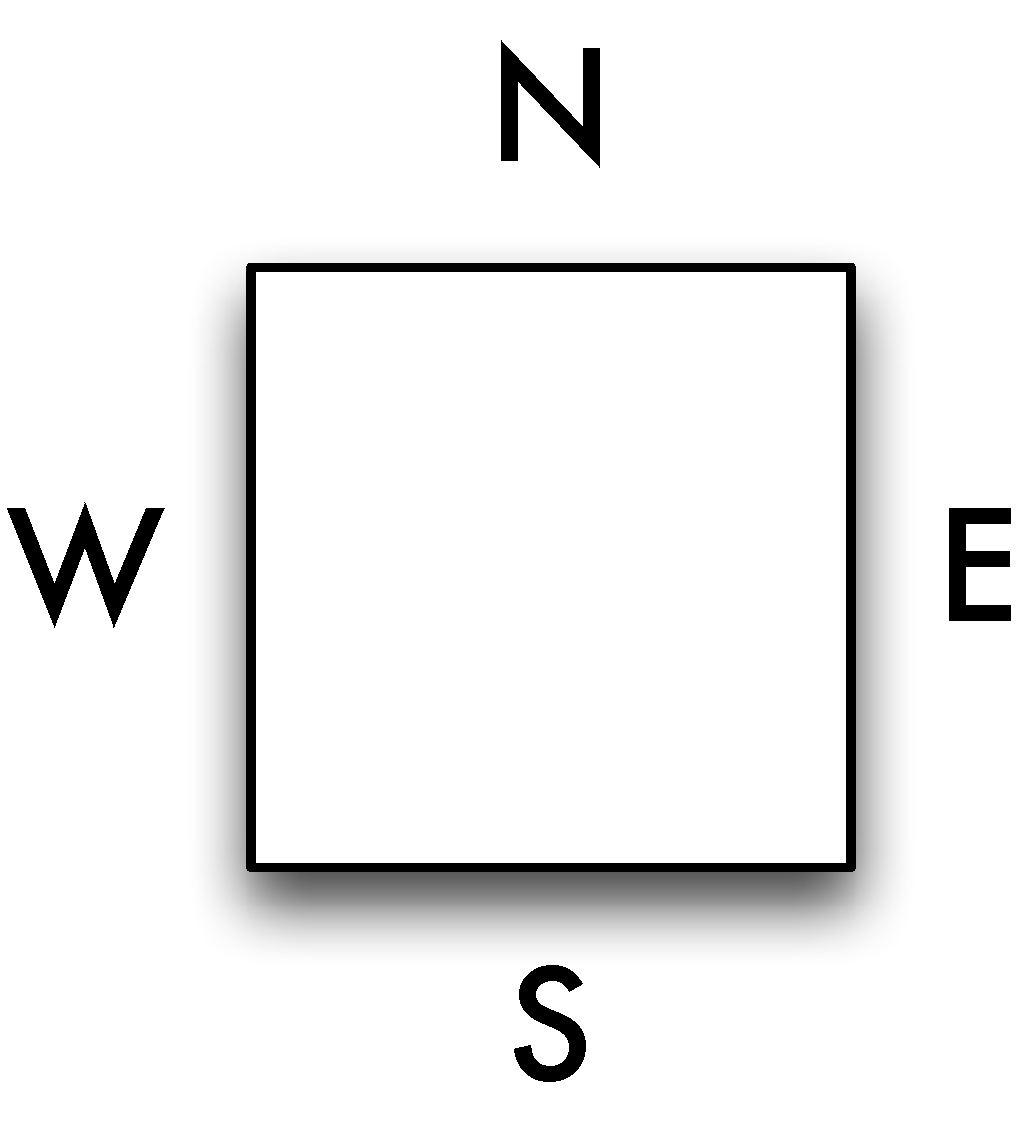
\includegraphics[width=2cm]{Pictures/NESW.pdf}
\end{wrapfigure}
\noindent
Many card games involve the idea of each player playing one card in turn, called a \emph{trick}.\index{trick} Traditionally for games like whist and bridge the players are called after the points of the compass: North, South, East and West. The play is in clockwise order: if East is the player to start (to \emph{lead}) then the players South, West and North follow in that order.

\begin{exercise}

\item
Define a type \texttt{Player} to represent the four players.

\end{exercise}

\noindent
There is an important rule about how players should choose cards to play.
A player should \emph{follow suit}: that is, if they can, they must play a card from the same suit as the card that was led (the card played by the person starting). A player can only play from a different suit if she has no cards left in the suit that was led.

\begin{wrapfigure}[12]{r}{3cm}
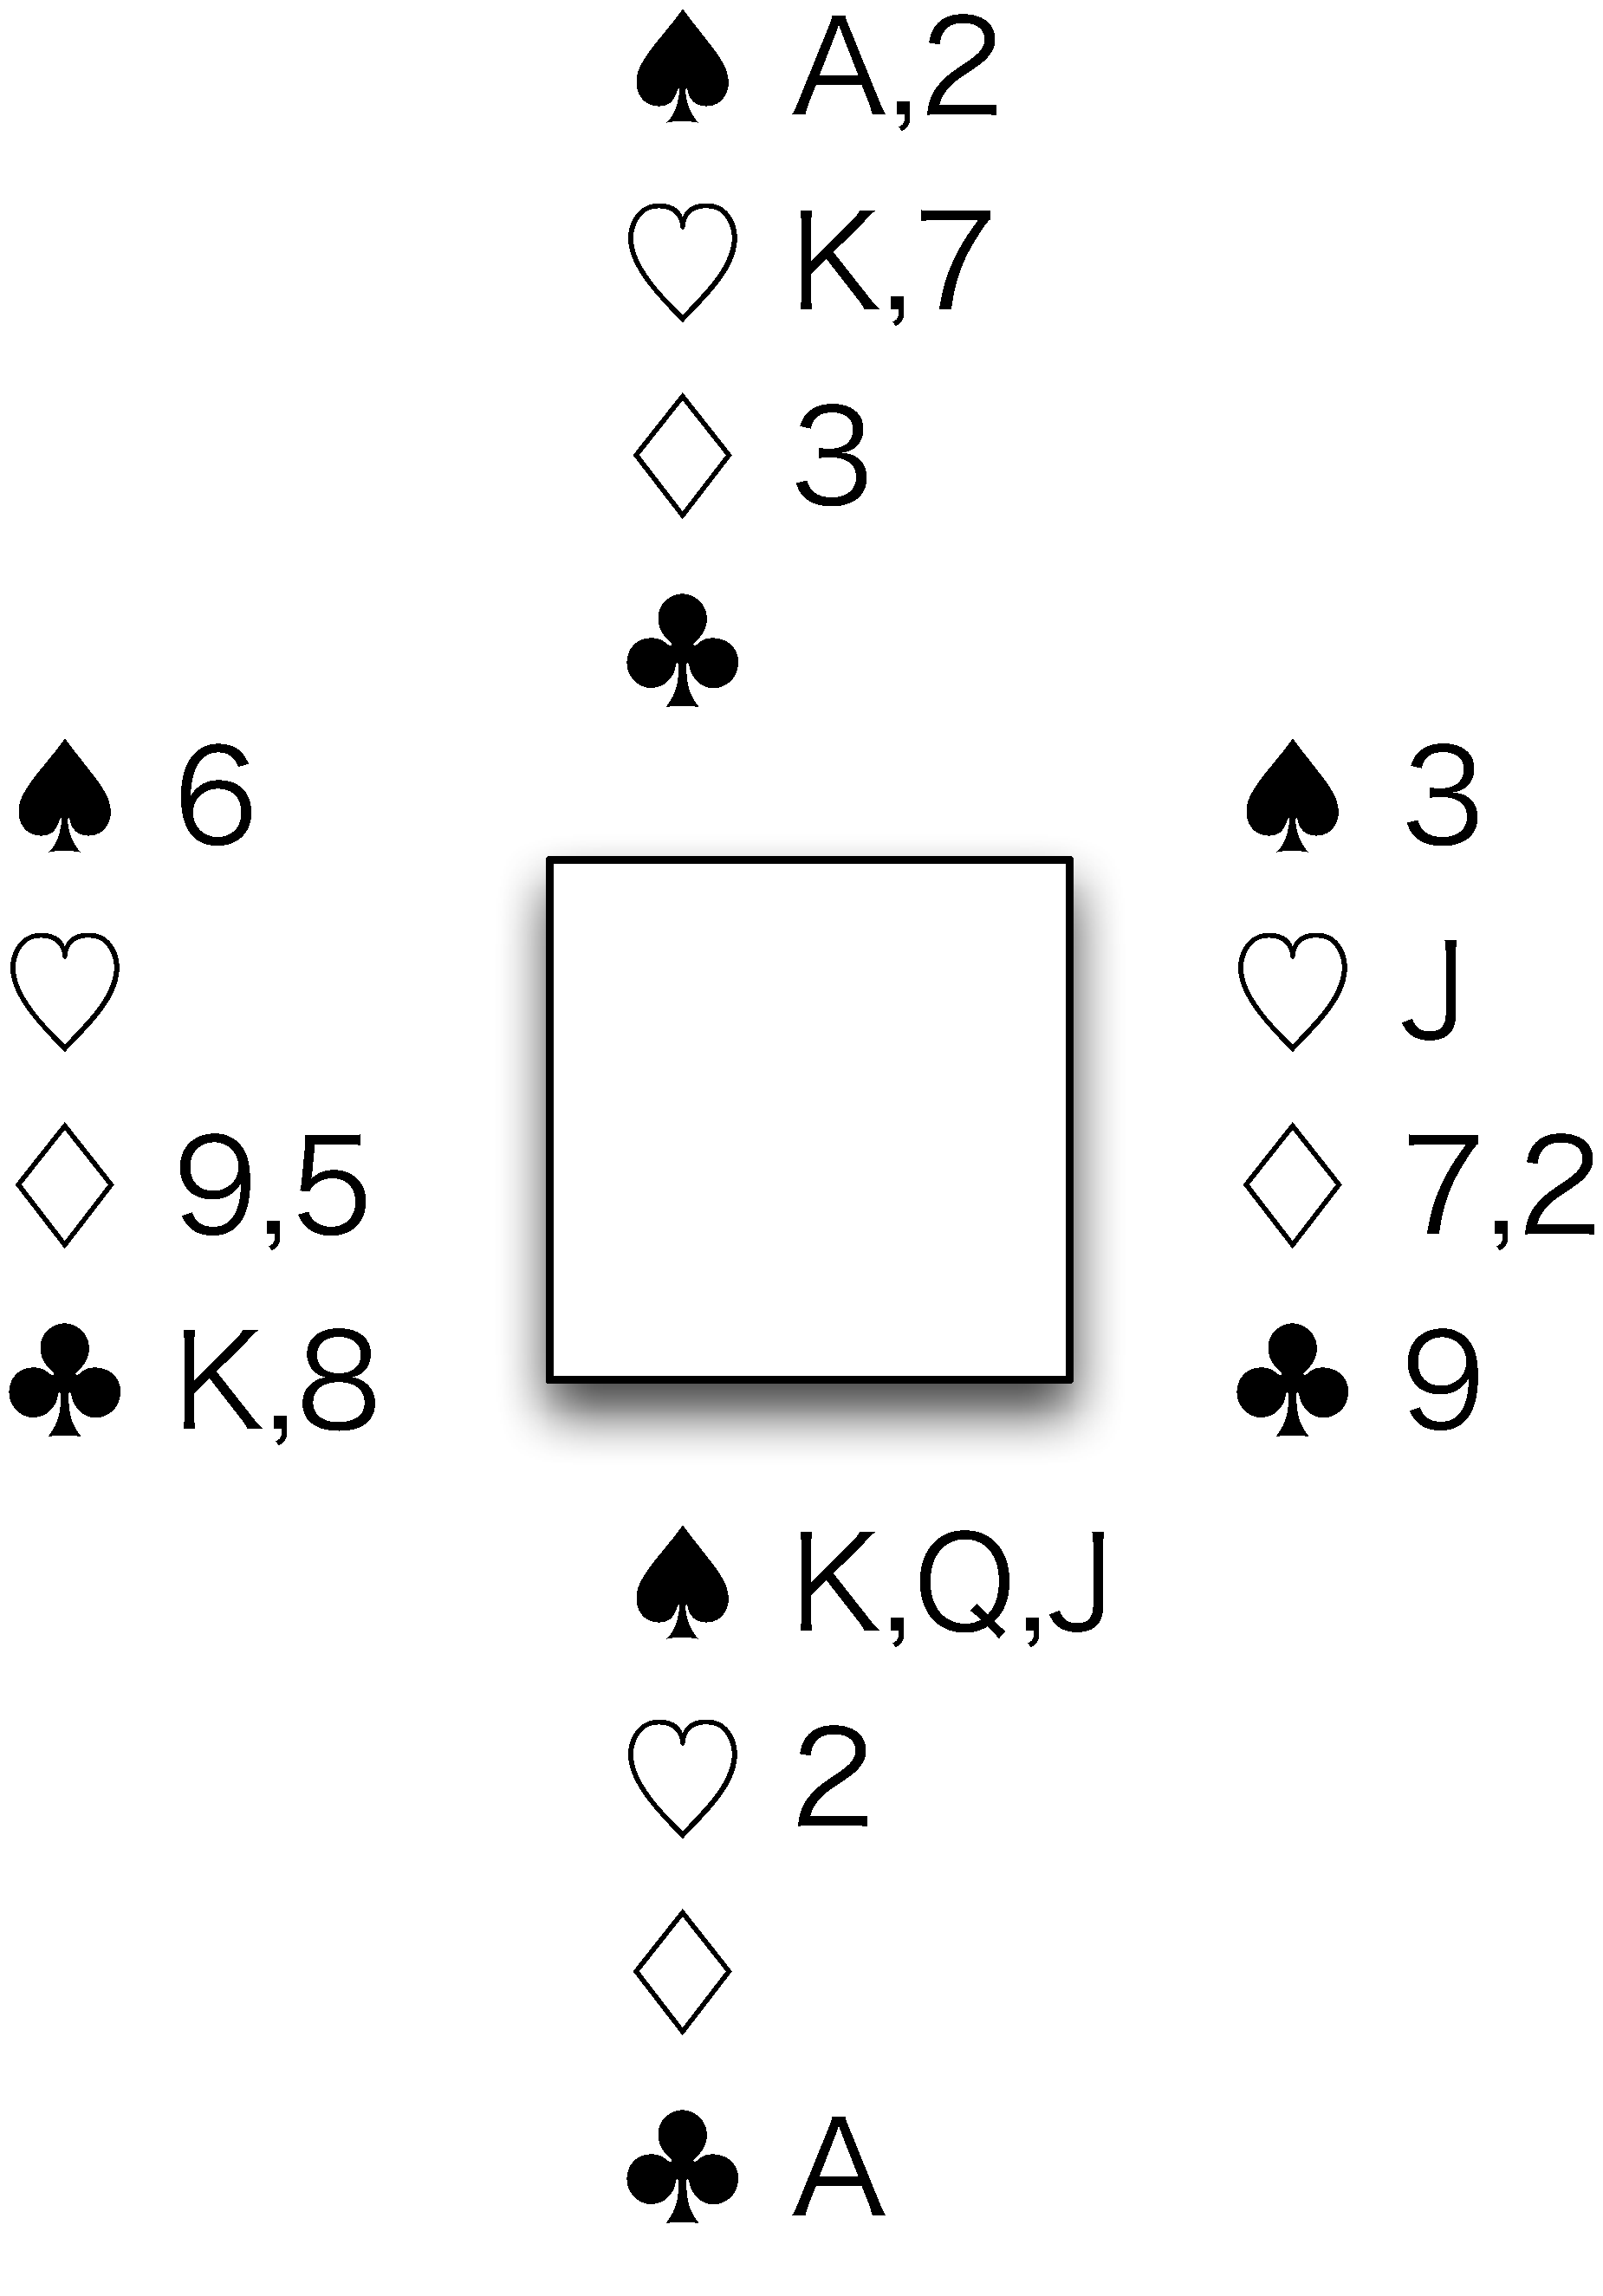
\includegraphics[width=3cm]{Pictures/Hand1.pdf}
\end{wrapfigure}
Let's have a look at an example. Suppose that each of the players has five cards left, as shown to the right. Suppose also that East is to lead and that she plays the Jack of Hearts.  
South has no choice: he has to play the 2 of Hearts. West has no Hearts, so she can choose any other card to play. Finally, North has a choice of two Hearts: the King or the 7, let's suppose that he plays the King.

Who wins the trick? Let's suppose first that there is no trump suit. The highest Heart will win the trick, and that's the King. Why Hearts? Because a Heart was led by East.\\
\hspace*{0.5cm} If there is a \emph{trump}\index{trump} suit, then the highest trump card wins if any trumps have been played, but remember that you can only play a trump if you're unable to follow suit. If Spades were trumps in this case, then West could win the trick by playing the 6 of Spades, no one else can play a trump as they are able to follow suit.

\begin{exercises}

\item
How would you represent a trick? Define a type \texttt{Trick}, using either a \texttt{type} or a \texttt{data} definition. Remember that you need to know which player has played which card, and also who led.

\item
Define a function
\begin{alltt}
winNT :: Trick -> Player
\end{alltt}
which decides the winner of a trick, assuming that there is no trump suit.

\item
Define a function
\begin{alltt}
winT :: Suit -> Trick -> Player
\end{alltt}
which decides the winner of a trick, assuming that there is a trump suit, which is passed in as the first argument.

\item
Define a type \texttt{Hand} which represents the collection of cards held by a player at one point during a game. In the earlier example, the hand held by North is \spade A, 2; \heart K, 7; \dia 3 (and no \club{} cards). 

\item Define a type \texttt{Hands} which describes the hands held by the four players at one point in the game. This should represent the four hands shown in the diagram above, for example.

\item
Define a function
\begin{alltt}
checkPlay :: Hands -> Trick -> Bool
\end{alltt}
which checks whether the play in a particular trick is both \emph{possible} and \emph{legal}. It should be possible in the sense that the card played by each player (given in the \texttt{Trick}) should be in their hand, as given in the \texttt{Hands}. It should be legal in following the rule that players should \emph{follow suit} if they can.
\end{exercises}

\noindent
What does a game look like? As there are 52 cards, when dealt to four players this results in each player receiving 13 cards. There will therefore be thirteen tricks played. In whist and bridge pairs of players -- North/South and East/West -- play together, so in an game of 13 tricks one side or the other will win.

\begin{exercises}

\item
Define a type \texttt{Team} to represent the two teams North/South and East/West. Define a function 
\begin{alltt}
winnerNT :: [Trick] -> Team
\end{alltt} 
which will give the winning team from the list of tricks, assuming that there are no trumps. Also define the function
\begin{alltt}
winnerT :: Suit -> [Trick] -> Team
\end{alltt} 
where the trump suit is passed in as the first argument.

\item {[Harder]}
Define a function 
\begin{alltt}
checkPlay :: [Trick] -> Bool
\end{alltt}
which checks whether the play in each trick is both \emph{possible} and \emph{legal}.
\emph{Hint:} you will need to deduce the hand in each case from the cards played subsequently: once you have done this, you can use \texttt{checkPlay} as defined earlier.

\end{exercises}
\index{extended exercise!card games|)}

 
\begin{summary}

This chapter has shown how the combination of list comprehensions and the built-in
functions from the prelude give us a powerful repertoire of tools with
which to build definitions over particular list types. This was evident
in the \texttt{Picture} example as well as in the case studies, and
these also gave an opportunity to see the way in which a larger program
was built as a collection of related functions.
returning a member of the same list type. The example in Section \ref{cardGames} particularly emphasised the process of choosing types to represent the various entities in the domain in question.

Section \ref{HaskellLibs} contains vital information about the libraries available in Haskell, including how to download them, how to find out more about their contents and how to search for functions performing particular tasks. 

In the next chapter we'll find out about how to define functions over lists for ourselves.
\end{summary}

%\end{document}
